%###########################################################################
%
% Anhang
%
%###########################################################################
%\begin{appendix}
%\label{chap:Appendix}
%\chapter{Appendix A}
%\setcounter{chapter}{1}
%\addcontentsline{toc}{chapter}{Appendix}
%###########################################################################
% Anhang A
%###########################################################################
%\label{A}
%....


%\chapter{Appendix B}
%###########################################################################
% Anhang B
%###########################################################################
%\label{B}

%\pagebreak
%###########################################################################
%\end{appendix}


\renewcommand\thesection{\Alph{section}}
\renewcommand\thefigure{\thesection.\arabic{figure}}
\renewcommand{\thetable}{\thesection.\arabic{table}}
\setcounter{figure}{0}
\setcounter{table}{0}
\setcounter{section}{0}

\chapter*{Appendix}
\addcontentsline{toc}{chapter}{Appendix}

\label{chap:Appendix}

%-------------------------------------------------
\section{Structure and Mechanism} \label{sec:AppendixStructureandMechanism}
%-------------------------------------------------

\clearpage

\setcounter{figure}{0}
\setcounter{table}{0}

%-------------------------------------------------
\section{Locomotion} 
\label{app:Loco}
%-------------------------------------------------

\subsection{Locomotion Design Drivers}
\label{app:DesignDrivers}


%\begin{figure}[htb] 
%  \centering
%     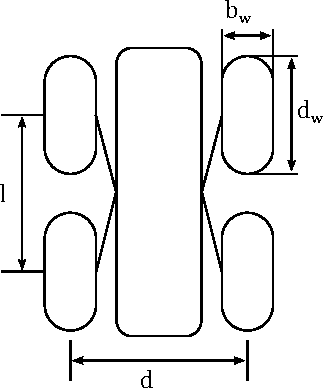
\includegraphics[width=1\textwidth]{Media/Geometries.pdf}
%  \caption{Geometry parameters of the locomotion system. }
%  \label{fig:Geo}
%\end{figure}

\begin{figure}[htb] 
  \centering
     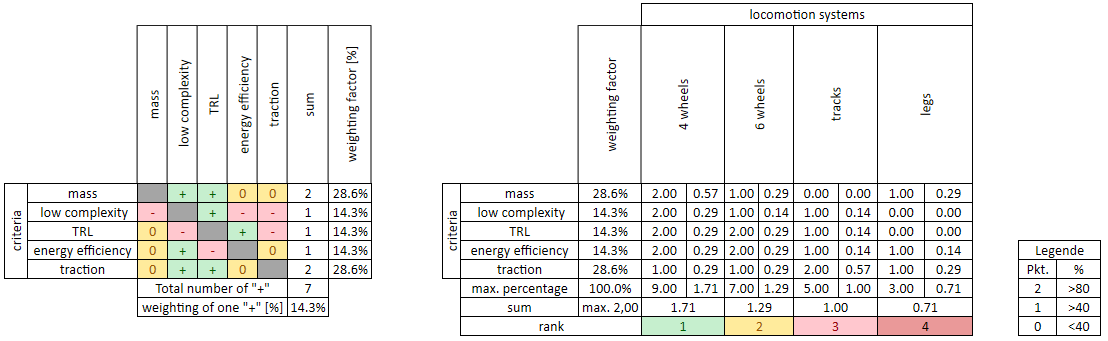
\includegraphics[width=1\textwidth]{Media/LocomotionTradeOff.png}
  \caption{Trade-off of the locomotion movement system. The criteria with the respective weighting factors are shown on the left. On the right side are the respective systems.}
  \label{fig:TradeOffLoco}
\end{figure}


\begin{figure}[htb] 
  \centering
     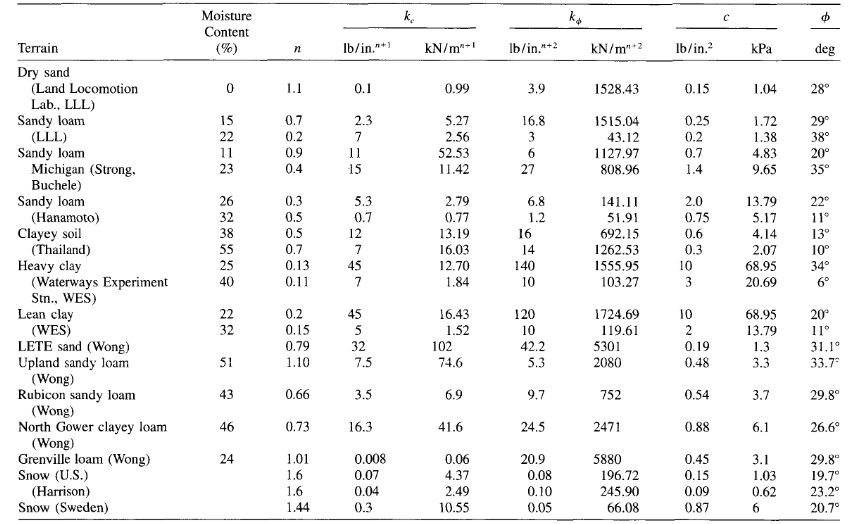
\includegraphics[width=1\textwidth]{Media/SoilParameters.png}
  \caption{Soil Parameters}
  \label{fig:SoilParameters}
\end{figure}


\begin{figure}[htb] 
  \centering
     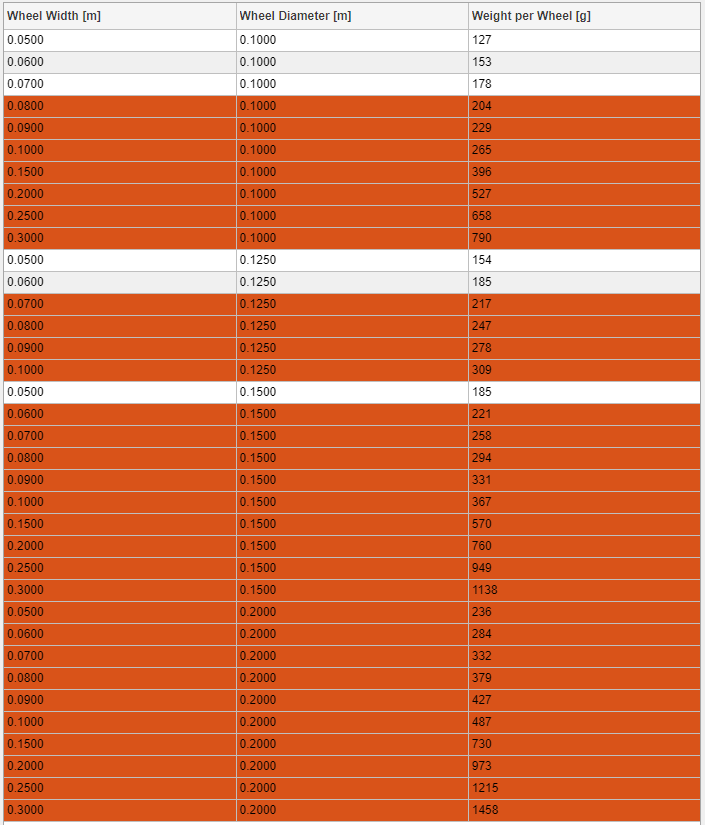
\includegraphics[width=1\textwidth]{Media/Dimensions-WeightLimits.png}
  \caption{Various wheel dimensions respective to the weight. Rows highlighted in red are not considered further for system design due to the limit of 200 g weight per wheel.}
  \label{fig:DimensionsLoco}
\end{figure}

\subsubsection*{Mean Maximum Pressure}
\label{app:MMP}


\begin{figure}[htb] 
  \centering
     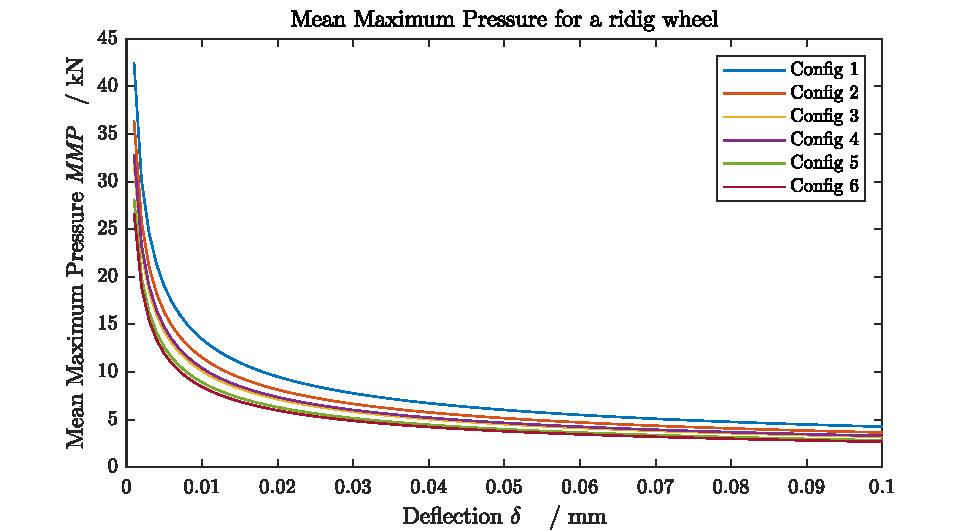
\includegraphics[width=1\textwidth]{Media/MMP for each Config.pdf}
  \caption{}
  \label{fig:MMP}
\end{figure}

\begin{figure}[htb] 
  \centering
     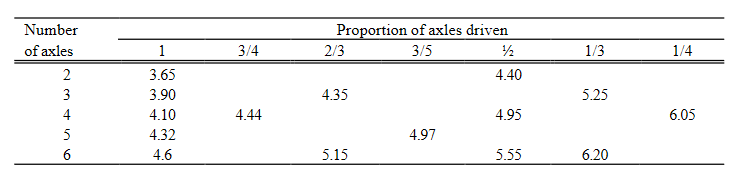
\includegraphics[width=1\textwidth]{Media/MMP_Param.png}
  \caption{Parameters for the mean maximum pressure for a wheeled rover.}
  \label{fig:MMP_param}
\end{figure}

\subsubsection*{Ackerman Steering}
\label{app:Ackerman}



\begin{table}[htb]
\centering
\caption{}
\begin{adjustbox}{max width=\textwidth}
\begin{tabular}[l]{lccc}

	\toprule
		\multicolumn{1}{l}{Steering Angle} & \multicolumn{1}{c}{Mode 1} & \multicolumn{1}{c}{Mode 2} & \multicolumn{1}{c}{Mode 3} \\
		
	\midrule
	
	
	\(\theta_\text{o}\)	&	&	&	\\	
	
	\(\theta_\text{o}\) &	&	&	\\


	\bottomrule

\end{tabular}
\end{adjustbox}
\label{tab:Ackerman}
\end{table}


\clearpage

\setcounter{figure}{0}
\setcounter{table}{0}

%-------------------------------------------------
\section{Electrical Power System} \label{sec:AppendixEPS}
%-------------------------------------------------
\begin{table}[htb]
\centering
\caption{INSPIRE battery parameters.}
\begin{tabular}{|c|c|}
\hline
\multicolumn{2}{|c|}{\textbf{SAFT 176065 xlr} \cite{SAFTBatteries.2018}}                                                                \\ \hline
\multicolumn{2}{|c|}{\textbf{Configuration:}}                                                                 \\ \hline
Battery Configuration                                                           & $3s4p$                        \\ \hline
Cells in Sereis $s$ N [-]                                                       & $3$                           \\ \hline
Cells in Parallel $p$ M [-]                                                     & $4$                           \\ \hline
\multicolumn{2}{|c|}{\textbf{Cell Parameters:}}                                                               \\ \hline
Typical Cell Capacity   [Ah]                                                    & $6.8$                         \\ \hline
Nominal Cell Voltage [V]                                                        & $3.65$                        \\ \hline
Nominal Cell Capacity [Wh]                                                      & $24.8$                        \\ \hline
Typical Cell Mass [kg]                                                          & $0.15$                        \\ \hline
Energy Density [Wh/kg]                                                     & $165.33$                      \\ \hline
\multicolumn{2}{|c|}{\textbf{Actual Battery Configuration Parameters:}}                                       \\ \hline
Battery Voltage $V_\text{Batt}$ [V]                                             & $10.95$                        \\ \hline
Battery Nominal Capacity $E_\text{Batt}$ [Wh]                                   & $297.6$                       \\ \hline
Battery Mass  [$kg$]                                                               & $1.8$                         \\ \hline
\textbf{Battery Mass} $m_\text{Batt}$ (incl. $10\%$ Margin) [kg]                                         & \textbf{1.98}                        \\ \hline
\multicolumn{2}{|c|}{\textbf{Configruation according to ECSS reliability restrictions and margins included:}} \\ \hline
Battery Configuration                                                           & $3s3p$                        \\ \hline
Cells in Sereis $s$ N [-]                                                       & $3$                           \\ \hline
Cells in Parallel $p$ M [-]                                                     & $3$                           \\ \hline
Battery Voltage $V_\text{Batt}$ [V]                                             & $10.95$                       \\ \hline
Battery Nominal Capacity $E_\text{Batt}$ [Wh]                                   & $231.60$                       \\ \hline
$30\%$ Margin on Energy Content                                                 & $0.3$                         \\ \hline
\textbf{Battery Nominal Capacity} $E_\text{Batt}$ incl. Margin [Wh]                      & \textbf{156.24}                      \\ \hline
Useable Energy Density [Wh/kg]                                              & $78.91$                       \\ \hline
\end{tabular}
\label{tab:battery}
\end{table}

\begin{figure}[htb]
{\centering
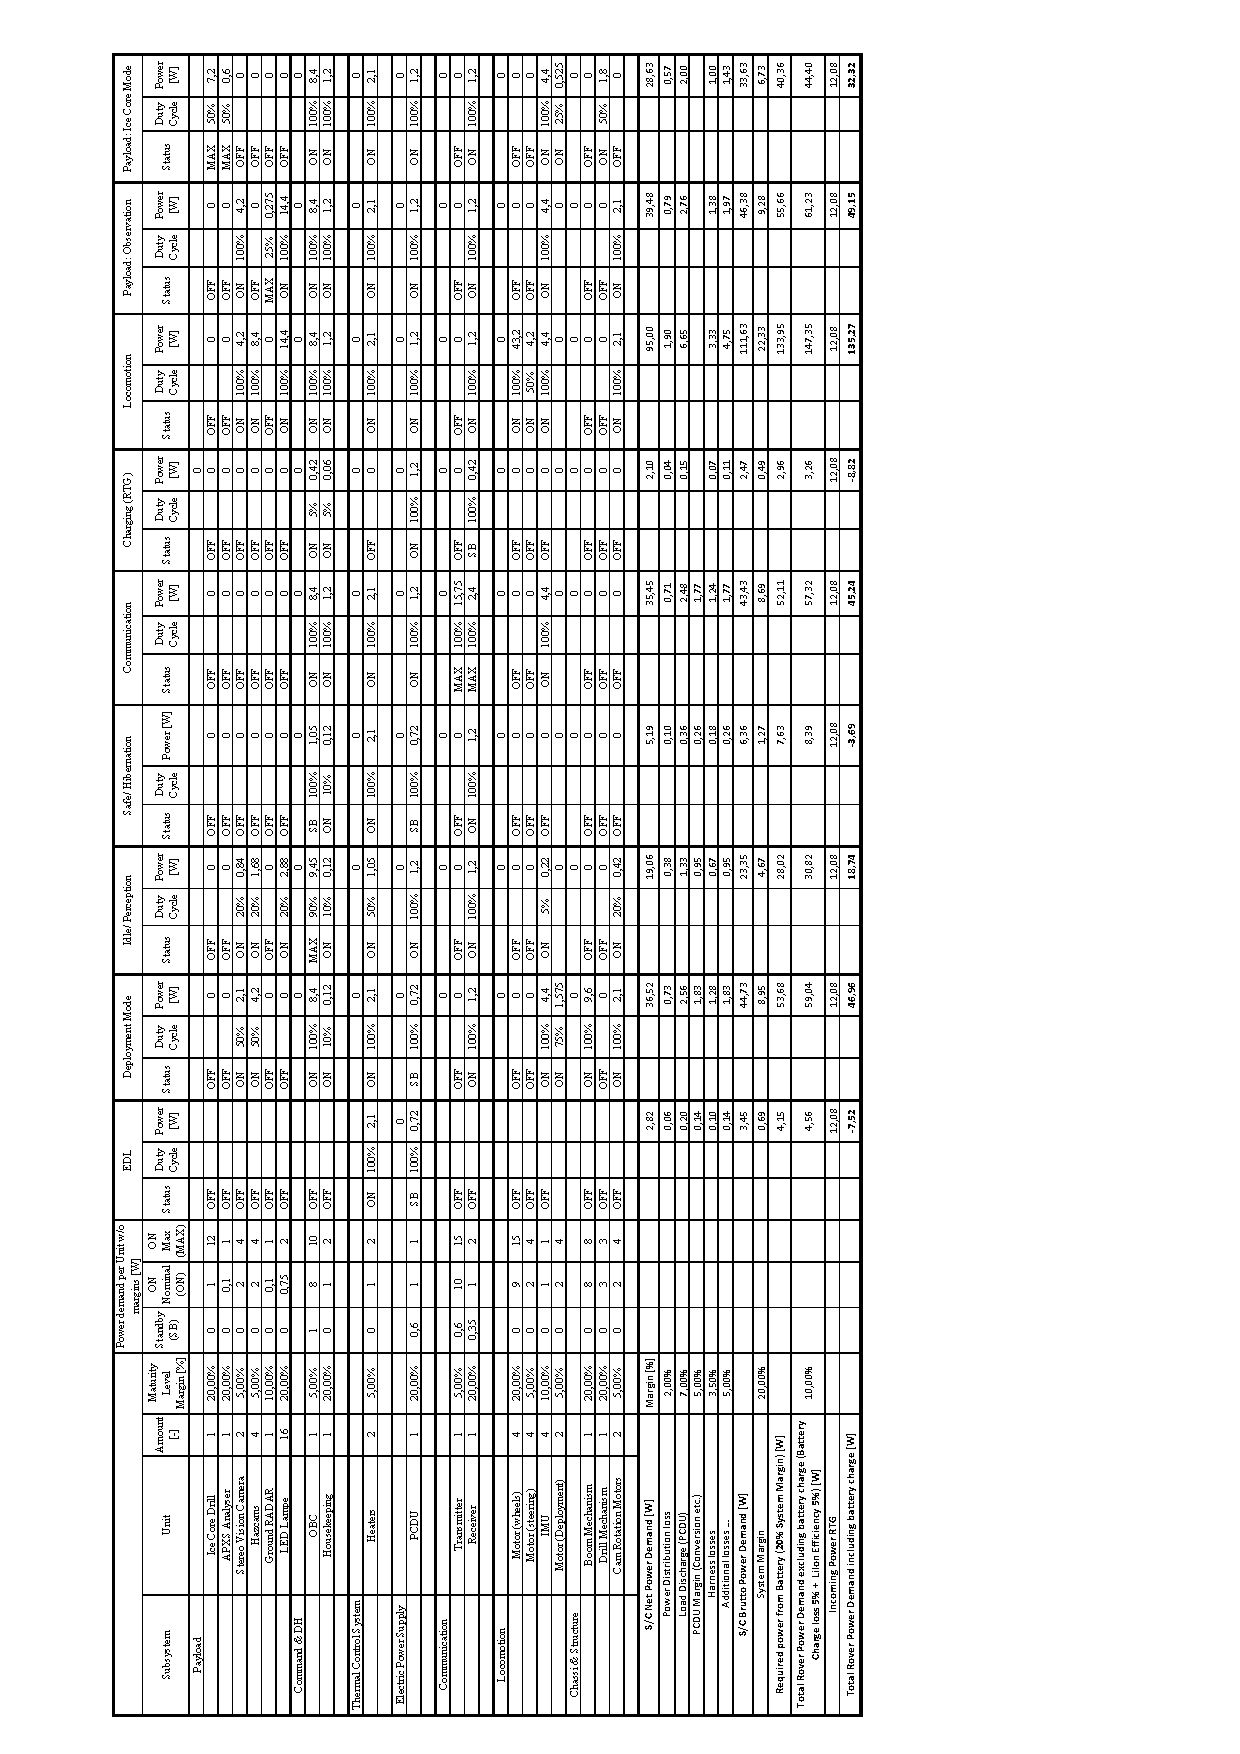
\includegraphics[width=1.0\textwidth]{Media/budgeteps}
\caption{Holistic Power Budget of INPSIRE.}
\label{tab:powerbudgetcomplete}
}
\end{figure}

\clearpage

\setcounter{figure}{0}
\setcounter{table}{0}

%-------------------------------------------------
\section{Communications} 
\label{sec:AppendixCOM}
%-------------------------------------------------

\subsection{Link Budget}
\label{app:LinkBudget}

Link budget considerations are performed under the conservative assumptions listed in \autoref{tab:lb-param}. \\

\begin{table}[h]
\centering
\begin{tabular}{llclll}
\hline
Parameter                        & Value  & Unit	       & Symbol        & Source                       &  \\ \hline
Rover                            &        &            &               &                              &  \\ \hline\hline
antenna Gain           		     & 2      & {[}dB{]}   & ${G}_{R}$  	   & omnidirectional LGA          &  \\
output power        	         & 1      & {[}W{]}    & ${P}_{R}$  	   &                              &  \\
line loss               	     & 0,6    & {[}dB{]}   & ${L}_{l1}$ 	   & FLP                          &  \\ \hline
Path                             &        &            &               &                              &  \\ \hline\hline
R2L polarisation loss            & 0,3    & {[}dB{]}   & ${L}_{p}$ 	   & FLP                          &  \\
free space loss                  & 117,55 & {[}$m^3${]}& ${L}_{s}$  	   &                              &  \\
atmospheric loss                 & 0      & {[}dB{]}   & ${L}_{a}$	   & negligible atmosphere        &  \\ \hline
Lander                           &        &            &               &                              &  \\ \hline\hline
antenna Gain             		 & 1      & {[}dB{]}   & ${G}_{L}$	   & conservative estimation      &  \\
output power        	         & 5      & {[}W{]}    & ${P}_{L}$  	   & conservative estimation      &  \\
pointing Loss  		             & 0      & {[}dB{]}   & ${n/a}$       & omnidirectional LGA          &  \\
line Loss  		                 & 0,6    & {[}dB{]}   & ${L}_{l2}$	   & FLP                          &  \\
eff. noise temperature           & 300    & {[}K{]}    & ${T}_{s}$	   & worst case E-bay temperature &  \\ \hline
Demodulation \& Uncertain Losses &        &            &               &                              &  \\ \hline\hline
eff. data rate                   & 5000   & {[}kbps{]} & ${R}$         & 50 \% of max. data rate                            &  \\
FEC coding                       & none   & {[}-{]}    & ${n/a}$       &                              &  \\
technical degradation            & 1      & {[}dB{]}   & ${L}_{i1}$    & FLP                          &  \\
implementation loss              & 1      & {[}dB{]}   & ${L}_{i1}$	   & FLP                          &  \\
                                 &        &            &               &                              & 
\end{tabular}
\caption{Transmission link parameters}
\label{tab:lb-param}
\end{table}

The free space loss ${L}_{s}$ [$m^3$] in \autoref{tab:lb-param} is calculated using the following correlation. 

\begin{equation}
	\centering
		{L}_{s} = {\frac{(4 \pi s)^2 \cdot c}{f}}
	\label{eqn:Ls}
\end{equation}

The signal travel distance {s} is assumed to be $s = 2000\ m$ which is in excess of the mission goal described in \autoref{chap:sc-output}. In accordance with X-Band communication the frequency {f} is set to a value of $f = 8,2\ GHz$. The parameter c represents the speed of light in vacuum. For simplification purposes $c = 3 \cdot 10^9\ \frac{m}{s}$ is assumed. \\ \\   
Combining the parameters from \autoref{tab:lb-param} the link budget is calculated using \autoref{eqn:EbzuN0}. For the simplification of \autoref{eqn:EbzuN0} the line losses for the rover ${L}_{l1}$ and lander ${L}_{l2}$ are expressed as the sum ${L}_{l}$. In the same manner technical degradation and implementation losses are combined to ${L}_{i}$. Atmospheric losses ${L}_{a}$ and pointing errors in \autoref{eqn:EbzuN0} are neglected due to a lack of atmosphere and the utilisation of omnidirectional low gain antennas. Parameter ${k}$ describes the Boltzmann constant.   

\begin{equation}
  \centering
		{\frac{{E}_{b}}{{N}_{0}}} = {P} - {L}_{l} + {G}_{R} - {10\cdot \log{{L}_{s}}} - {L}_{a} + {G}_{L} + {10\cdot \log{k}} - {10\cdot \log{{T}_{s}}} - {10\cdot \log{{R}}} - {L}_{i}
	\label{eqn:EbzuN0}
\end{equation}


\autoref{eqn:EbzuN0} and the conservative assumptions from \autoref{tab:lb-param} results in an energy per bit over noise $\frac{{E}_{b}}{{N}_{0}} = 10,59\ dB$. The complete link budget can be found in \autoref{fig:LB-R2L}. \\
Referencing \autoref{fig:BitErrorRate} a Bit Error Rate of $10^{-4}$ can be achieved in the downlink path, which is considered sufficient for a first assessment. Optionally a FEC code can be implemented in later design phases.\\

Using the same parameters listed in \autoref{tab:lb-param} leads to a $\frac{{E}_{b}}{{N}_{0}} = 50,56\ dB$ corresponding to a Bit Error Rate of potentially less than $10^{-6}$. Therefore the downlink does not contribute to the design decisions. The complete link budget for the uplink path can be found in \autoref{fig:LB-L2R}.

\begin{figure}[h]
	\centering
  		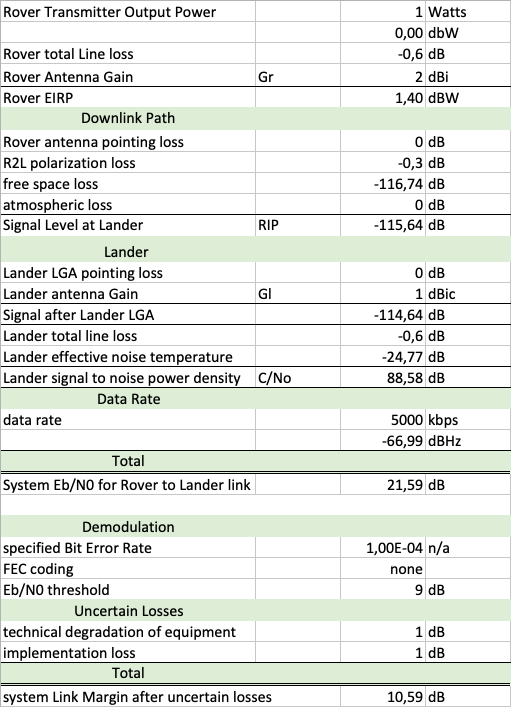
\includegraphics[width=0.9\textwidth]{Media/LB-RovertoLander.png}
  \caption{Rover to Lander complete downlink budget.}
  \label{fig:LB-R2L}
\end{figure}

\begin{figure}[h]
	\centering
  		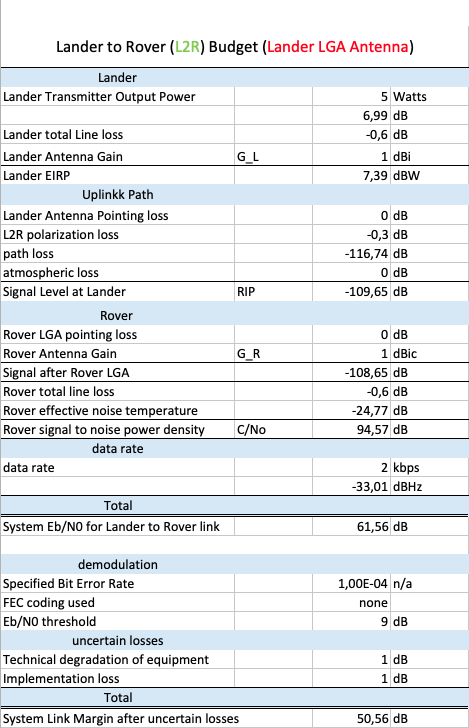
\includegraphics[width=0.9\textwidth]{Media/LB-LandertoRover.png}
  \caption{Lander to Rover complete uplink budget.}
  \label{fig:LB-L2R}
\end{figure}

\begin{figure}[h]
	\centering
  		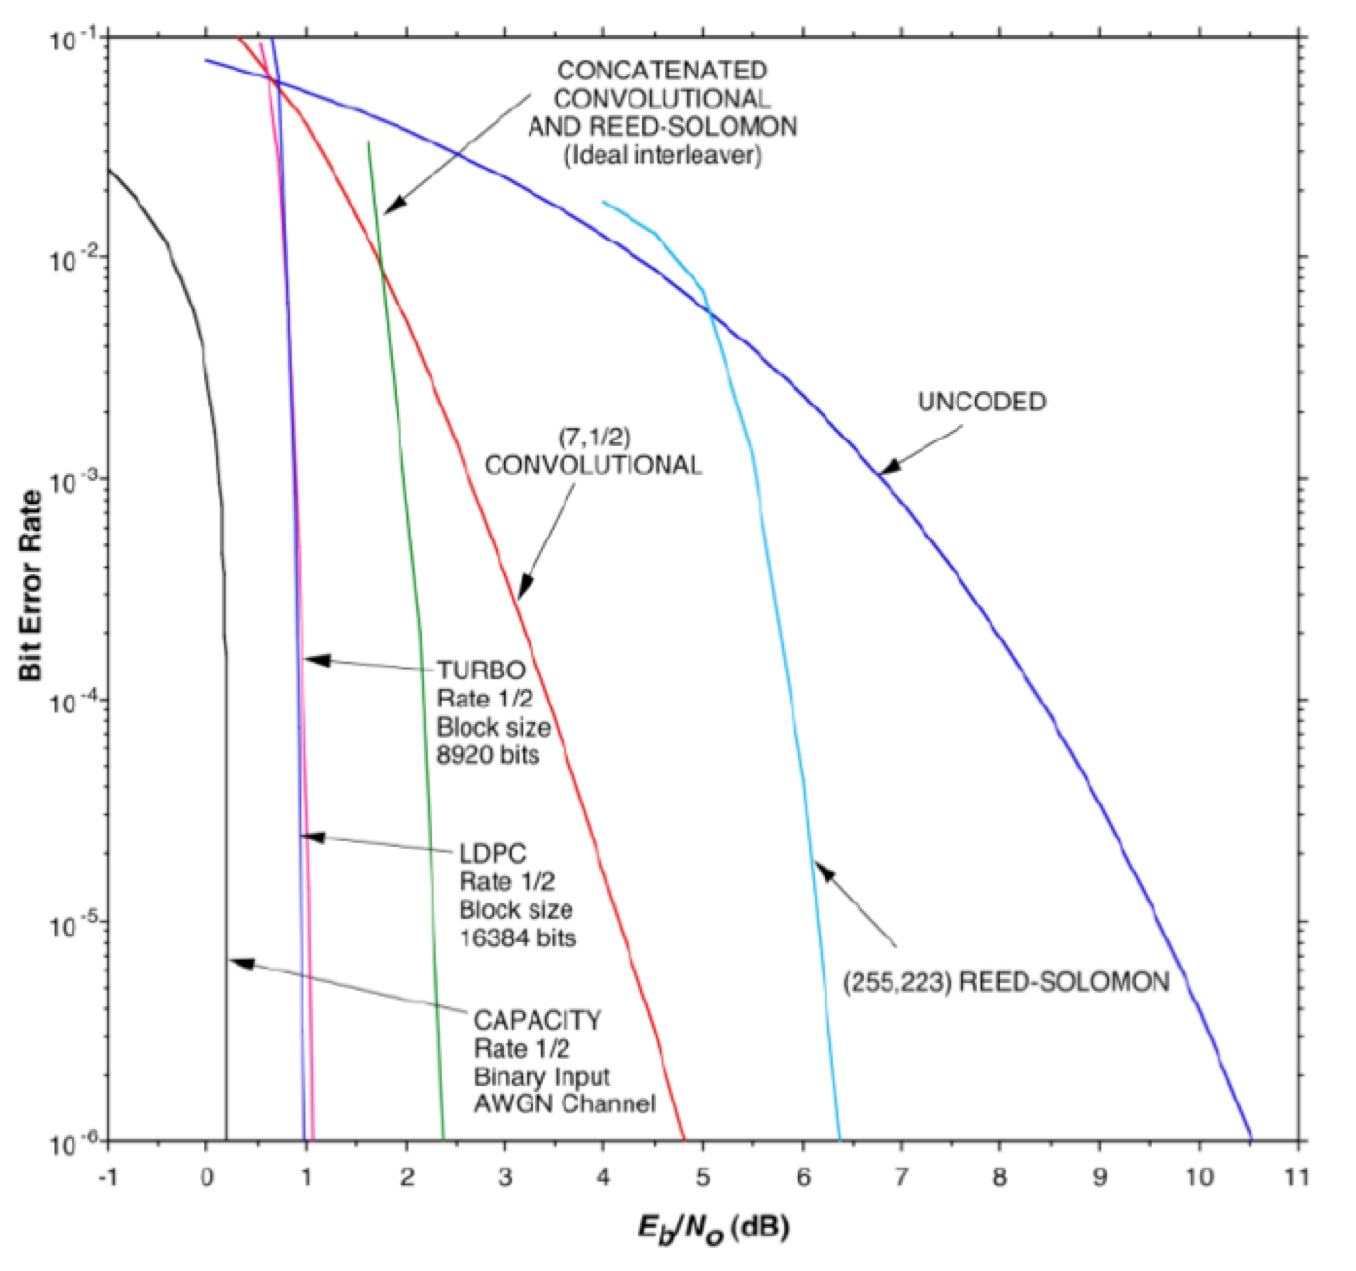
\includegraphics[width=0.9\textwidth]{Media/Bit_Error_Rate.png}
  \caption{Bit Error Rate for different FEC codes}
  \label{fig:BitErrorRate}
\end{figure}

\subsection{Mission Data Output}
\label{app:MissionDataOutput}

The analysis of the mission data concept for memory capacity and transmission times is focuses on the payload camera and Hazcams as images require far more data than telemetry or other payload data. \\

In a first assumption 420 images per day are stored and transmitted. Considering the sensor resolution of $2048\times2048$ pixels and a bit depth per pixel of 10 bit of the (CAMERA REFERENCE), a file size of 42 Mbit per image is assumed.\\
To calculate the message size in \autoref{tab:TimePerPic}, it is assumed that a transmission frame consists of 10264 bits including a payload frame of maximum 8840 bits (FLP VORELESUNG).   

\begin{table}[h]
\centering
\begin{tabular}{llllll}
File Type & Compression    & File Size  & Message Size & Data Rate & Tx t per File \\ \hline\hline
image     & none           & 42 Mbit    & 48,77 Mbit   & 5 Mbit    & 8,12 s        \\
image     & HIREW          & 23,52 Mbit & 27,31 Mbit   & 5 Mbit    & 5,45 s        \\ \hline
\end{tabular}
\caption{Comparison of transmission times per image (message frame bits included)}
\label{tab:TimePerPic}
\end{table}

\begin{table}[h]
\centering
\begin{tabular}{lllll}
File per tal & Compression & File Size  & Total Data & Tx time    \\ \hline\hline
420          & none        & 42 Mbit    & 2,21 GB    & 56,9 Min.  \\
420          & HIREW       & 23,52 Mbit & 1,22 GB    & 38,23 Min. \\ \hline
\end{tabular}
\caption{Transmission time and total data output per mission day}
\label{tab:Tx-tptal}
\end{table}

The HIREW compression algorithm is suggested for the mission considering a high average compression of 0,56 \% and a high compression speed of 123 Mbit/s for grayscale and 104,4 Mbit/s for RGB image files (COMPRESSSION PAPER REFERENCE). 

\subsection{Communications Trade Off}
\label{app:Com_TrOff}

\subsubsection{Transmitter Selection}
% Transmitter Trade off
\begin{figure}[h]
     \centering
     \begin{subfigure}[b]{0.49\textwidth}
         \centering
         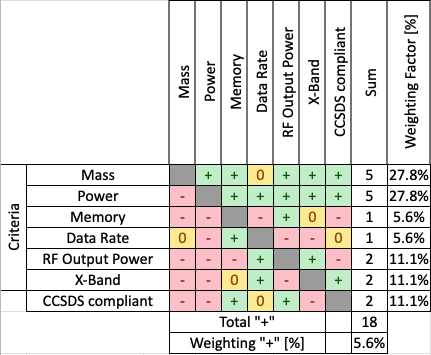
\includegraphics[width=\textwidth]{Media/Trade_off/Transmitter/Weighting_trans.png}
         \caption{Weighting of selection criteria for the transmitter.}
         \label{fig:Weighting_trans}
     \end{subfigure}
     \hfill
     \begin{subfigure}[b]{0.49\textwidth}
         \centering
         \includegraphics[width=\textwidth]{Media/Trade_off/Transmitter/Values_trans.png}
         \caption{Comparison of optional transmitters.}
         \label{fig:Values_trans}
     \end{subfigure}
     \hfill
     \begin{subfigure}[b]{0.49\textwidth}
         \centering
         \includegraphics[width=\textwidth]{Media/Trade_off/Transmitter/TradeOff_trans.png}
         \caption{Transmitter trade off.}
         \label{fig:TradeOff_trans}
     \end{subfigure}
     \hfill
     \caption{Transmitter Trade off for the Communication subsystem.}
     \label{TrOff_Trans}
\end{figure}

\subsubsection{Receiver Trade Off}
%Receiver Trade Off
\begin{figure}[h]
     \centering
     \begin{subfigure}[b]{0.49\textwidth}
         \centering
         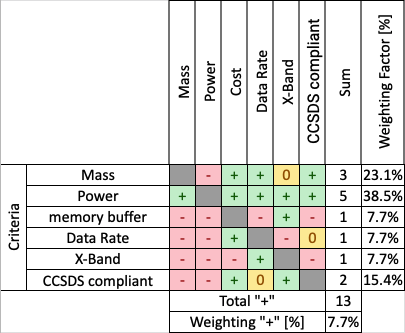
\includegraphics[width=\textwidth]{Media/Trade_off/Receiver/Weighting_Rec.png}
         \caption{Weighting of selection criteria for the receiver.}
         \label{fig:Weighting_Rec}
     \end{subfigure}
     \hfill
     \begin{subfigure}[b]{0.49\textwidth}
         \centering
         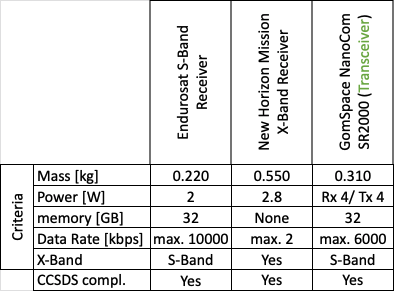
\includegraphics[width=\textwidth]{Media/Trade_off/Receiver/Values_Rec.png}
         \caption{Comparison of optional receivers.}
         \label{fig:Values_Rec}
     \end{subfigure}
     \hfill
     \begin{subfigure}[b]{0.49\textwidth}
         \centering
         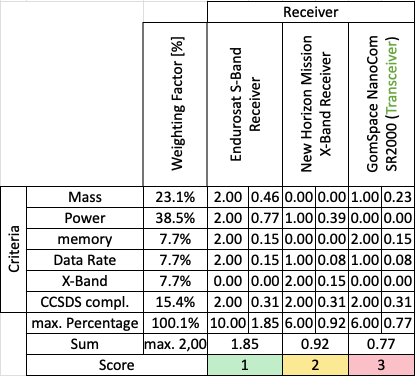
\includegraphics[width=\textwidth]{Media/Trade_off/Receiver/TradeOff_Rec.png}
         \caption{Receiver trade off.}
         \label{fig:TradeOff_Rec}
     \end{subfigure}
     \hfill
     \caption{Receiver Trade off for the Communication subsystem.}
     \label{TrOff_Trans}
\end{figure}

\subsubsection{Antenna Trade Off}
%Antenna Trade Off
\begin{figure}[h]
     \centering
     \begin{subfigure}[b]{0.49\textwidth}
         \centering
         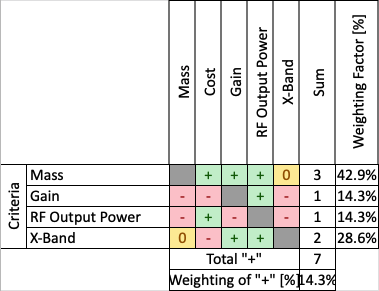
\includegraphics[width=\textwidth]{Media/Trade_off/Antenna/Weighting_Ant.png}
         \caption{Weighting of selection criteria for the antenna.}
         \label{fig:Weighting_Rec}
     \end{subfigure}
     \hfill
     \begin{subfigure}[b]{0.49\textwidth}
         \centering
         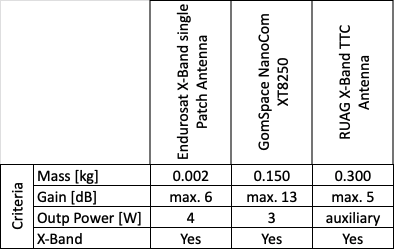
\includegraphics[width=\textwidth]{Media/Trade_off/Antenna/Values_Ant.png}
         \caption{Comparison of optional antenna.}
         \label{fig:Values_Rec}
     \end{subfigure}
     \hfill
     \begin{subfigure}[b]{0.49\textwidth}
         \centering
         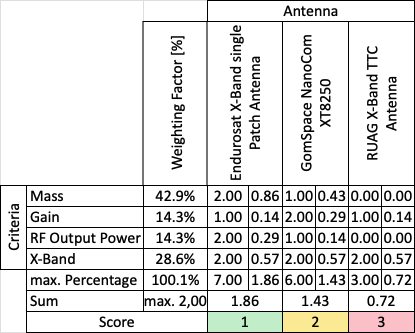
\includegraphics[width=\textwidth]{Media/Trade_off/Antenna/TradeOff_Ant.png}
         \caption{Antenna trade off.}
         \label{fig:TradeOff_Rec}
     \end{subfigure}
     \hfill
     \caption{Antenna trade off for the Communication subsystem.}
     \label{TrOff_Trans}
\end{figure}

\subsection{Command \& Data Handling Trade Off}

\subsubsection{OBC Trade Off}
%OBC Trade Off
\begin{figure}[h]
     \centering
     \begin{subfigure}[b]{0.49\textwidth}
         \centering
         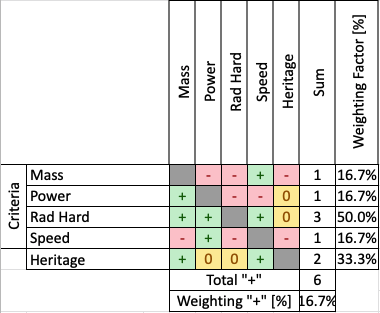
\includegraphics[width=\textwidth]{Media/Trade_off/OBC/Weighting_OBC.png}
         \caption{Weighting of selection criteria for the OBC.}
         \label{fig:Weighting_Rec}
     \end{subfigure}
     \hfill
     \begin{subfigure}[b]{0.49\textwidth}
         \centering
         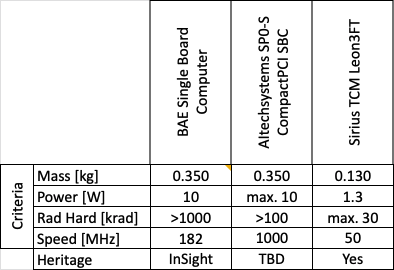
\includegraphics[width=\textwidth]{Media/Trade_off/OBC/Values_OBC.png}
         \caption{Comparison of optional single board computers.}
         \label{fig:Values_Rec}
     \end{subfigure}
     \hfill
     \begin{subfigure}[b]{0.49\textwidth}
         \centering
         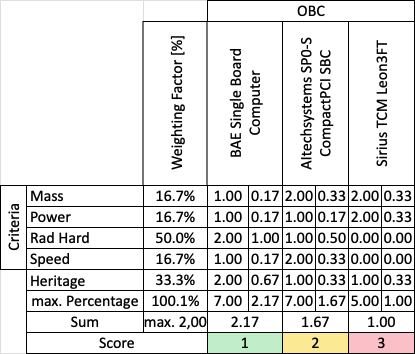
\includegraphics[width=\textwidth]{Media/Trade_off/OBC/TradeOff_OBC.png}
         \caption{Antenna trade off.}
         \label{fig:TradeOff_Rec}
     \end{subfigure}
     \hfill
     \caption{OBC trade off for the Command \& Data Handling subsystem.}
     \label{TrOff_Trans}
\end{figure}

\clearpage

\setcounter{figure}{0}
\setcounter{table}{0}

%-------------------------------------------------
\section{Thermal Controls System} \label{sec:AppendixThermal}
%-------------------------------------------------
\subsection{Heat energy eqilibrium}  \label{sec:app_tcs_01}
The follwing equiations describe each node of the thermal network.
The input values were tanken from EPS, \autoref{sec:app_therm_2}, \autoref{sec:app_therm_3}, \autoref{sec:app_therm_4} respectively.

\begin{table}[H]
	\begin{tabular}{l@{\quad}l@{\qquad\qquad\qquad}l@{\quad}l}
		\multicolumn{4}{l}{\textit{Subscript} for eqilibrium:}\\[0.5em]
		Bay & Electrical Bay & Dr	& Drill\\
		Bo & Bogie & 	E,D & Drive Engine\\
		Cam & Camera & E,S & Steer Engine\\
		Ch & Chassis & WF & Wheel Fork\\
	\end{tabular}

\end{table}

\underline{RTG:}

\begin{equation}
\begin{aligned}
0=\  &\dot{Q}_{RTG} +CON_1 \cdot (T_{Bay}-T_{RTG})+CON_2 \cdot (T_{Ch}-T_{RTG})+ \\[1em]
& + CON_5 \cdot (T_{Dr}-T_{RTG})+ CON_9 \cdot (T_{E,S}-T_{RTG})\\[1em]
& +   CON_12 \cdot (T_{E,D}-T_{RTG}) - \epsilon_{RTG}\cdot \sigma_b \cdot S_{RTG}\cdot T_{RTG}^4 \\[2em]
\end{aligned}
\end{equation}

\underline{Electric Bay:}\quad \small{Subscript\ \textit{Bay}}
\begin{equation}0=\  \dot{Q}_{Bay}+ CON_1 \cdot (T_{RTG}-T_{Bay})+ CON_3 \cdot (T_{Ch}-T_{Bay})  -\epsilon_{Bay}\cdot \sigma_b \cdot S_{Bay}\cdot T_{Bay}^4 \end{equation}\\
with: 
\begin{equation} \dot{Q}_{Bay} = \dot{Q}_{OBC} + \dot{Q}_{Tranceiver} +\dot{Q}_{Receiver} +\dot{Q}_{PCDU} \end{equation}\\

\underline{Drill \& Analyser:}
\begin{equation} 0= \ \dot{Q}_{Dr} +CON_4 \cdot (T_{Ch}-T_{Dr})+CON_5 \cdot (T_{RTG}-T_{Dr})   \end{equation} \\

\underline{Camera:}
\begin{equation}
\begin{aligned}
0=\  &  \dot{Q}_{Cam} + \dot{Q}_{RHU} +CON_6 \cdot (T_{Ch}-T_{Cam})+ \\[1em]
& +(CON_{14} +n_{S1}\cdot CON_{S1}) \cdot (T_{Rad}-T_{Cam})  - \epsilon_{Cam}\cdot \sigma_b \cdot S_{Cam}\cdot T_{Cam}^4 \\[2em]
\end{aligned}
\end{equation}

\underline{Radiator:}
\begin{equation}(CON_{14} +n_{S1}\cdot CON_{S1}) \cdot (T_{Cam}-T_{Rad}) - \epsilon_{Rad}\cdot \sigma_b \cdot S_{Rad}\cdot T_{Rad}^4= 0  \end{equation}  \\

\underline{Chassis:}
\begin{equation}
\begin{aligned}
0=\  &   \dot{Q}_{Radar}+\dot{Q}_{Hazcam}  +CON_2 \cdot (T_{RTG}-T_{Ch})+CON_3 \cdot (T_{Bay}-T_{Ch})+ \\[1em]
&  +CON_4 \cdot (T_{Drill}-T_{Ch})+ CON_6 \cdot (T_{Cam}-T_{Ch})+CON_7 \cdot (T_{Node_1}-T_{Ch}) +  \\[1em]
&  + \alpha_{Ch}\cdot [ S_0 \cdot (1+\rho_E) \cdot (S_{Ch1} \cdot \varphi_1  +S_{Ch2} \cdot \varphi_2 ) +   \epsilon_{E} \cdot \sigma_b \cdot S_{Ch3}\cdot T_{Surface}^4 ]-  \\[1em]
&   -\epsilon_{Ch}\cdot \sigma_b \cdot S_{Ch}\cdot T_{Ch}^4 \\[2em]
\end{aligned}
\end{equation}

\underline{Steer Engine:}
\begin{equation}
\begin{aligned}
0=\  &  4\cdot [\dot{Q}_{E,S} +(CON_8 +n_{S2}\cdot CON_{S2}) \cdot (T_{Node1}-T_{E,S})+ \\[1em]
&   +CON_9 \cdot (T_{RTG}-T_{E,S}) -\epsilon_{E,S}\cdot \sigma_b \cdot S_{E,S}\cdot T_{E,S}^4] \\[2em]
\end{aligned}
\end{equation}

\underline{Distribution Node 1:}
\begin{equation}
\begin{aligned}
0=\  &  4\cdot [CON_7 \cdot (T_{Ch}-T_{Node_1})+CON_8 \cdot (T_{E,S}-T_{Node_1})+ \\[1em]
&   +CON_10 \cdot (T_{Node_2}-T_{Node_1})] %\\[2em]
\end{aligned}
\end{equation}

\underline{Drive Engine:}
\begin{equation}
\begin{aligned}
0=\  &  4 \cdot [\dot{Q}_{E,D}+ (CON_{11}+n_{S3}\cdot CON_{S3}) \cdot (T_{Node_2}-T_{E,D})+ \\[1em]
&  + CON_{12} \cdot (T_{RTG}-T_{E,D})-\epsilon_{E,D}\cdot \sigma_b \cdot S_{E,D}\cdot T_{E,D}^4 ]  %\\[2em]
\end{aligned}
\end{equation}

\underline{Distribution Node 2:}
\begin{equation}
\begin{aligned}
0=\ & 4 \cdot [CON_{10} \cdot (T_{Node_1}-T_{Node_2})+CON_{11} \cdot (T_{E,D}-T_{Node_2})+   \\[1em]
&   +CON_{13} \cdot (T_{Ground}-T_{Node_2})  ]% \\[2em]
\end{aligned}
\end{equation}
\clearpage

\subsection{Heat conductance} \label{sec:app_therm_2}
\begin{table}[H]
	\centering
	\caption{Definition of heat conductance C between the nodes according to \autoref{fig:tcs_network}.}
	\begin{tabular}{l@{\qquad}cccc}
		\hline
		Name &  Linked Components &  \multicolumn{3}{c}{Geometry}\\ \hline
		& & & & \\[-0.75em]
		\textbf{Linkage} & \textbf{RTG} $\leftrightarrow$ \textbf{Chassis}  &  \multicolumn{3}{c}{\multirow{2}{*}{\adjustbox{valign=t}{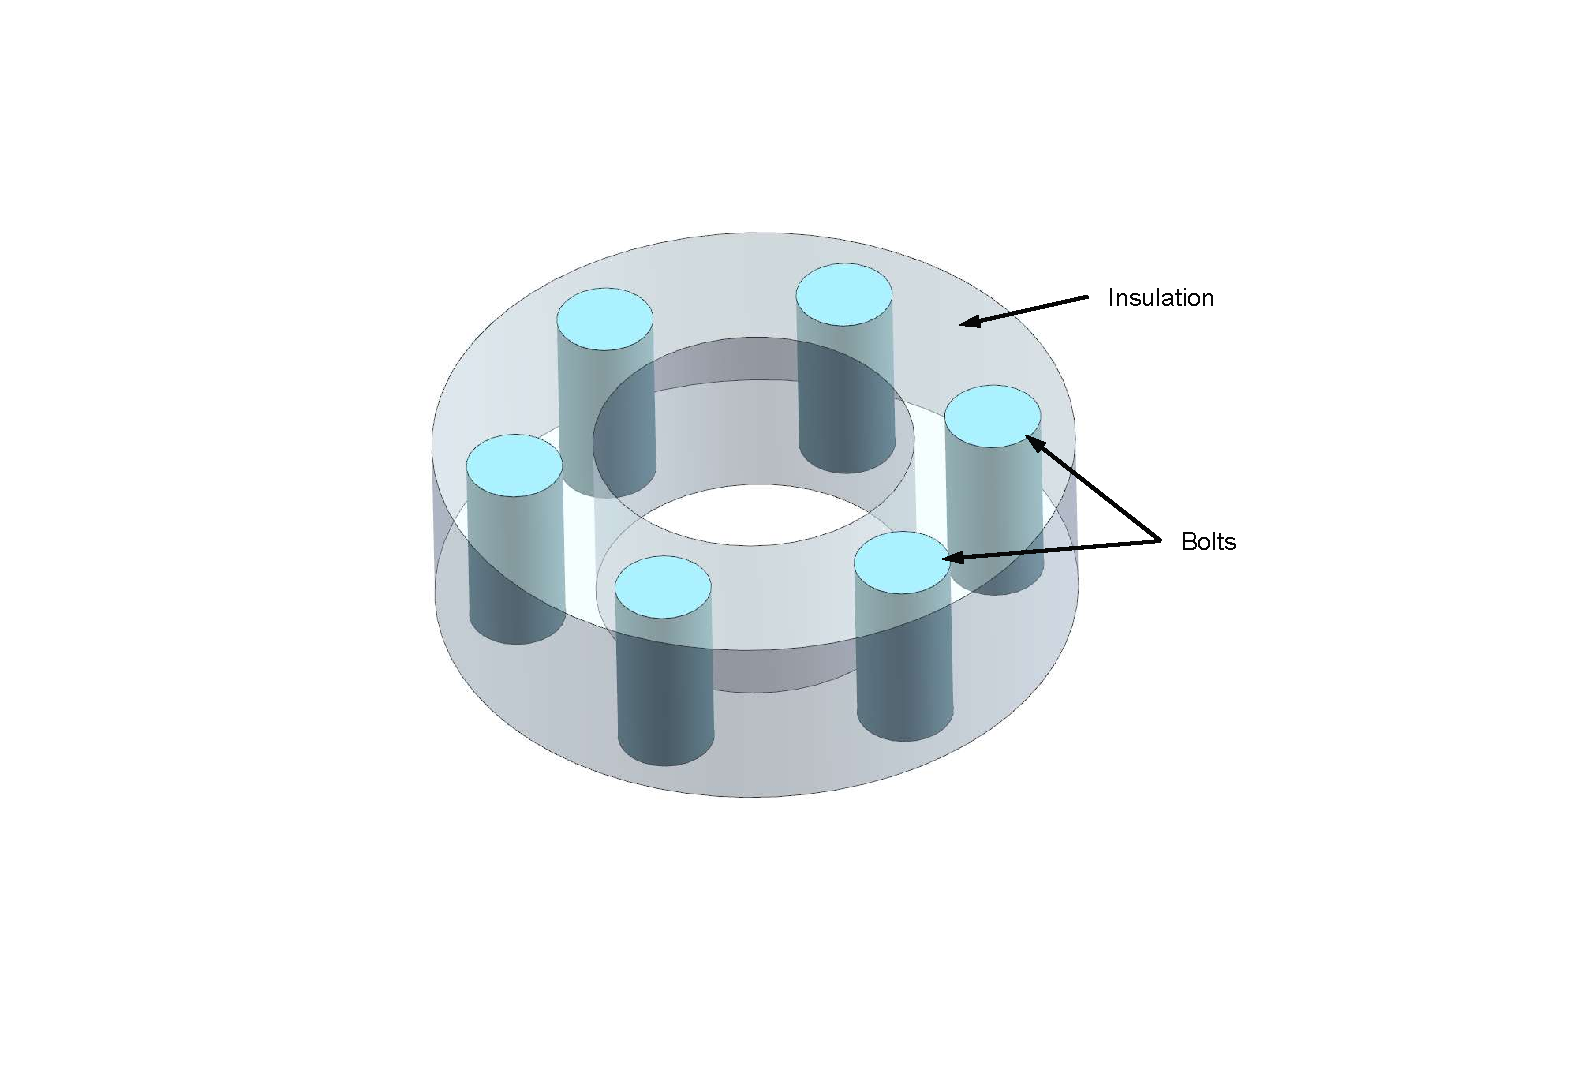
\includegraphics[width=0.3\textwidth]{Media/tcs_con_rtg}}}}  \\[1em]
		& & & &  \\
		\multicolumn{2}{l}{$CON_2= CON_{I}+n_{B}\cdot CON_{B}$} & & & \\[1em]
		\multicolumn{2}{l}{$CON_2= 1.50 \cdot 10^{-1}\ \frac{\W}{\K} $} & & &  \\[3em]
		\hline
		Part &  Cross section & Thickness  & Material & Amount \\ \hline
		& & & & \\[-0.75em]
		Insulation & $S_I=3'770\ \mm^2$ & $t_I=12\ \mm$ & Aerogel & 1 \\[0.5em]
		Bolts, M6 & $S_B=28.3\ \mm^2$ & $t_B=12\ \mm$ & Titan & 10 \\[5em]
		
		\hline
		Name &  Linked Components &  \multicolumn{3}{c}{Geometry}\\ \hline
		& & & & \\[-0.5em]
		\textbf{Linkage} & \textbf{EBay} $\leftrightarrow$ \textbf{Chassis}  &  \multicolumn{3}{c}{\multirow{2}{*}{\adjustbox{valign=t}{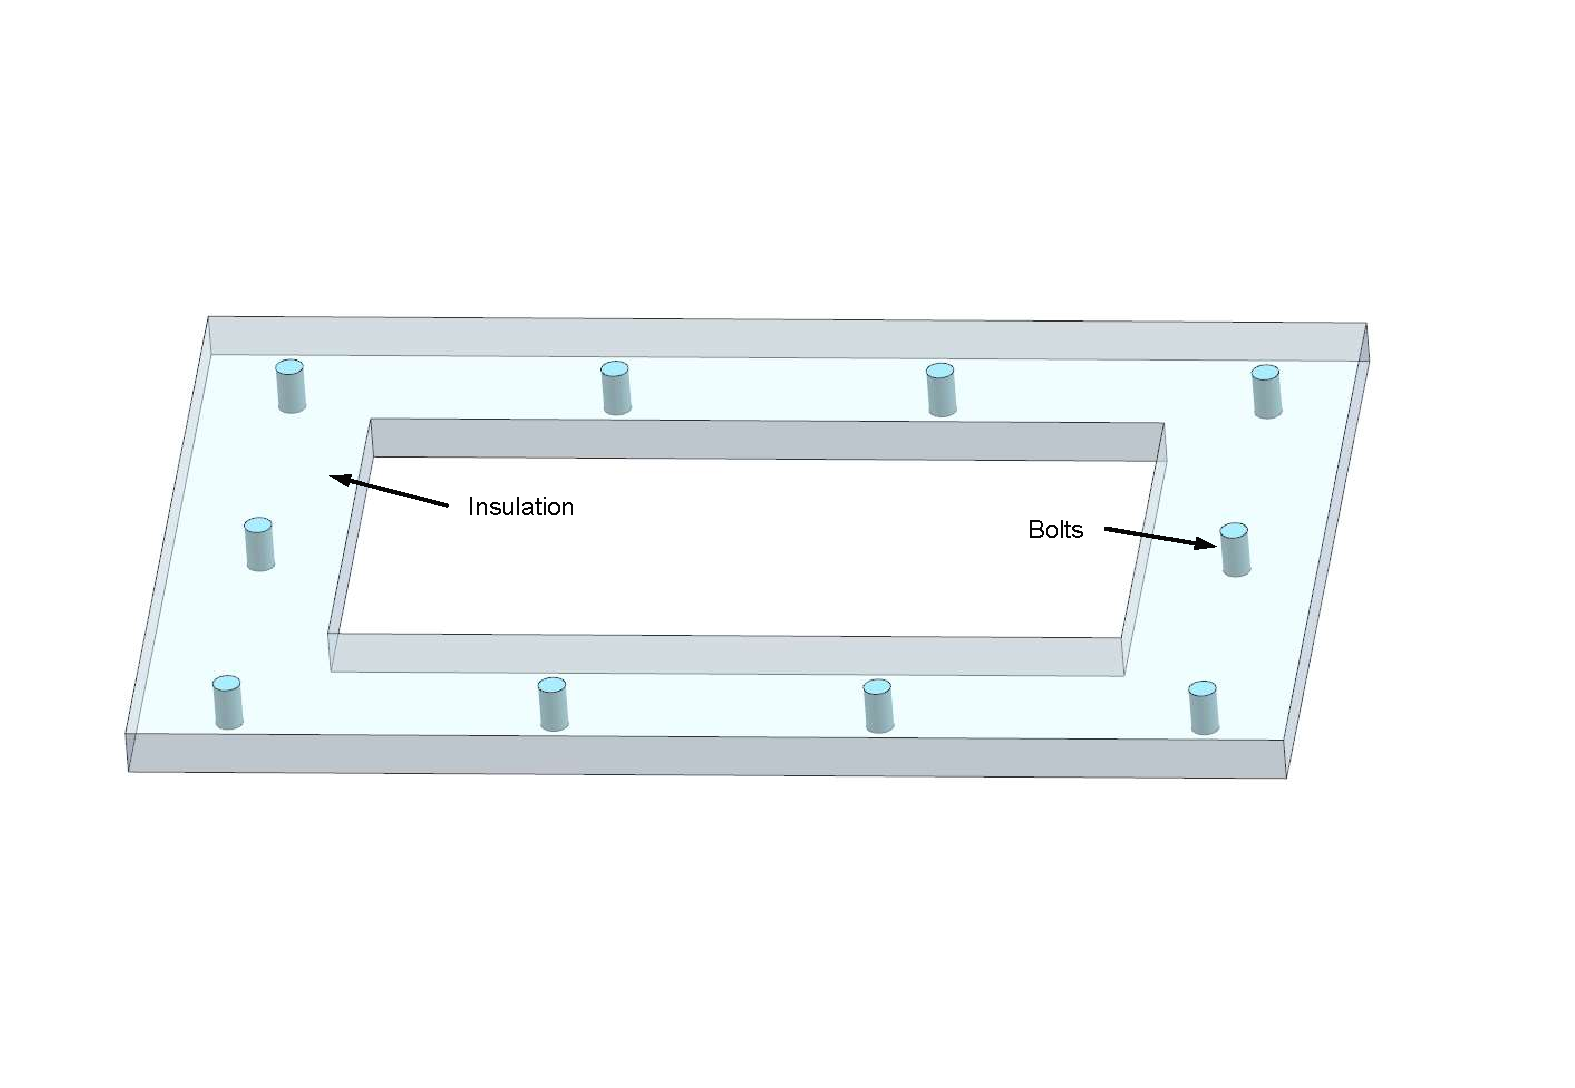
\includegraphics[width=0.5\textwidth]{Media/tcs_con_bay}}}}  \\[1em]
		& & & &  \\
		\multicolumn{2}{l}{$CON_3= CON_{I}+n_{B}\cdot CON_{B}$} & & &  \\[1em]
		\multicolumn{2}{l}{$CON_3= 2.80 \cdot 10^{-1}\ \frac{\W}{\K}$} & & & \\[3em]
		
		\hline
		Part &  Cross section & Thickness  & Material & Amount \\ \hline
		& & & & \\[-0.75em]
		Insulation & $S_I=27'120 \ \mm^2$ & $t_I=12\ \mm$ & Aerogel & 1 \\[0.5em]
		Bolts, M6 & $S_B=28.3 \ \mm^2$ & $t_B=12\ \mm$ & Titan & 10 \\	
	\end{tabular}
	\label{tab:tcs_nodes1}
\end{table}	

\begin{table}[H]
	\centering
	\caption{Definition of heat conductance $CON=\frac{1}{R}$ between the nodes according to \autoref{fig:tcs_network}.}
	\begin{tabular}{l@{\qquad}cccc}
				\hline
		Name &  Linked Components &  \multicolumn{3}{c}{Geometry}\\ \hline
		& & & & \\[-0.5em]
		\textbf{Linkage} & \textbf{Drill} $\leftrightarrow$ \textbf{Chassis}  &  \multicolumn{3}{c}{\multirow{2}{*}{\adjustbox{valign=t}{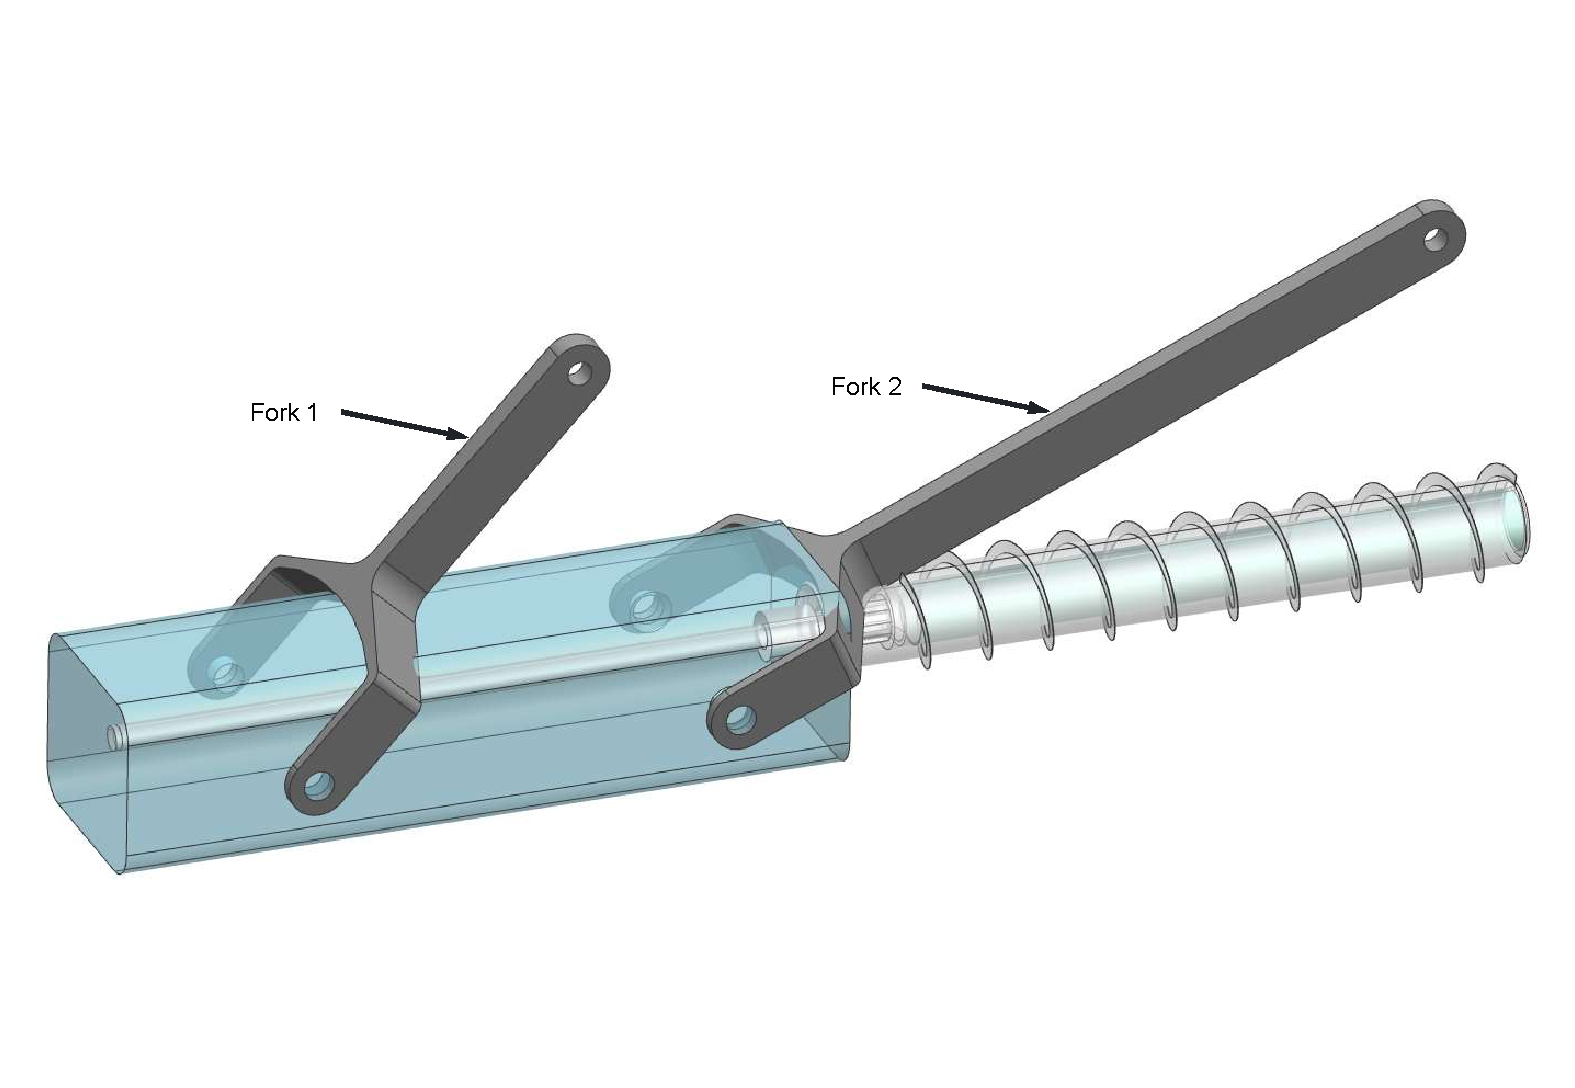
\includegraphics[width=0.55\textwidth]{Media/tcs_con_drill}}}}  \\[1em]
		& & & &  \\
		\multicolumn{2}{l}{$CON_{4}=CON_{F1}+CON_{F2} $} & & & \\[1em]
		\multicolumn{2}{l}{$CON_{4}= 1.56 \cdot 10^{-1}\ \frac{\W}{\K}$} & & & \\[4em]
		
		\hline
		Part &  Cross section & Length  & Material & Amount \\ \hline
		& & & & \\[-0.75em]
		Fork 1& $S_{F1}=40 \ \mm^2$ & $l_{F1}=90$ & Aluminium & 1 \\[0.5em]	
		Fork 1& $S_{F2}=40 \ \mm^2$ & $l_{F2}=150$ & Aluminium & 1 \\[5em]	
		
		
		\hline
		Name &  Linked Components &  \multicolumn{3}{c}{Geometry}\\ \hline
		& & & & \\[-0.5em]
		\textbf{Telescope} & \textbf{Camera} $\leftrightarrow$ \textbf{Chassis}  &  \multicolumn{3}{c}{\multirow{2}{*}{\adjustbox{valign=t}{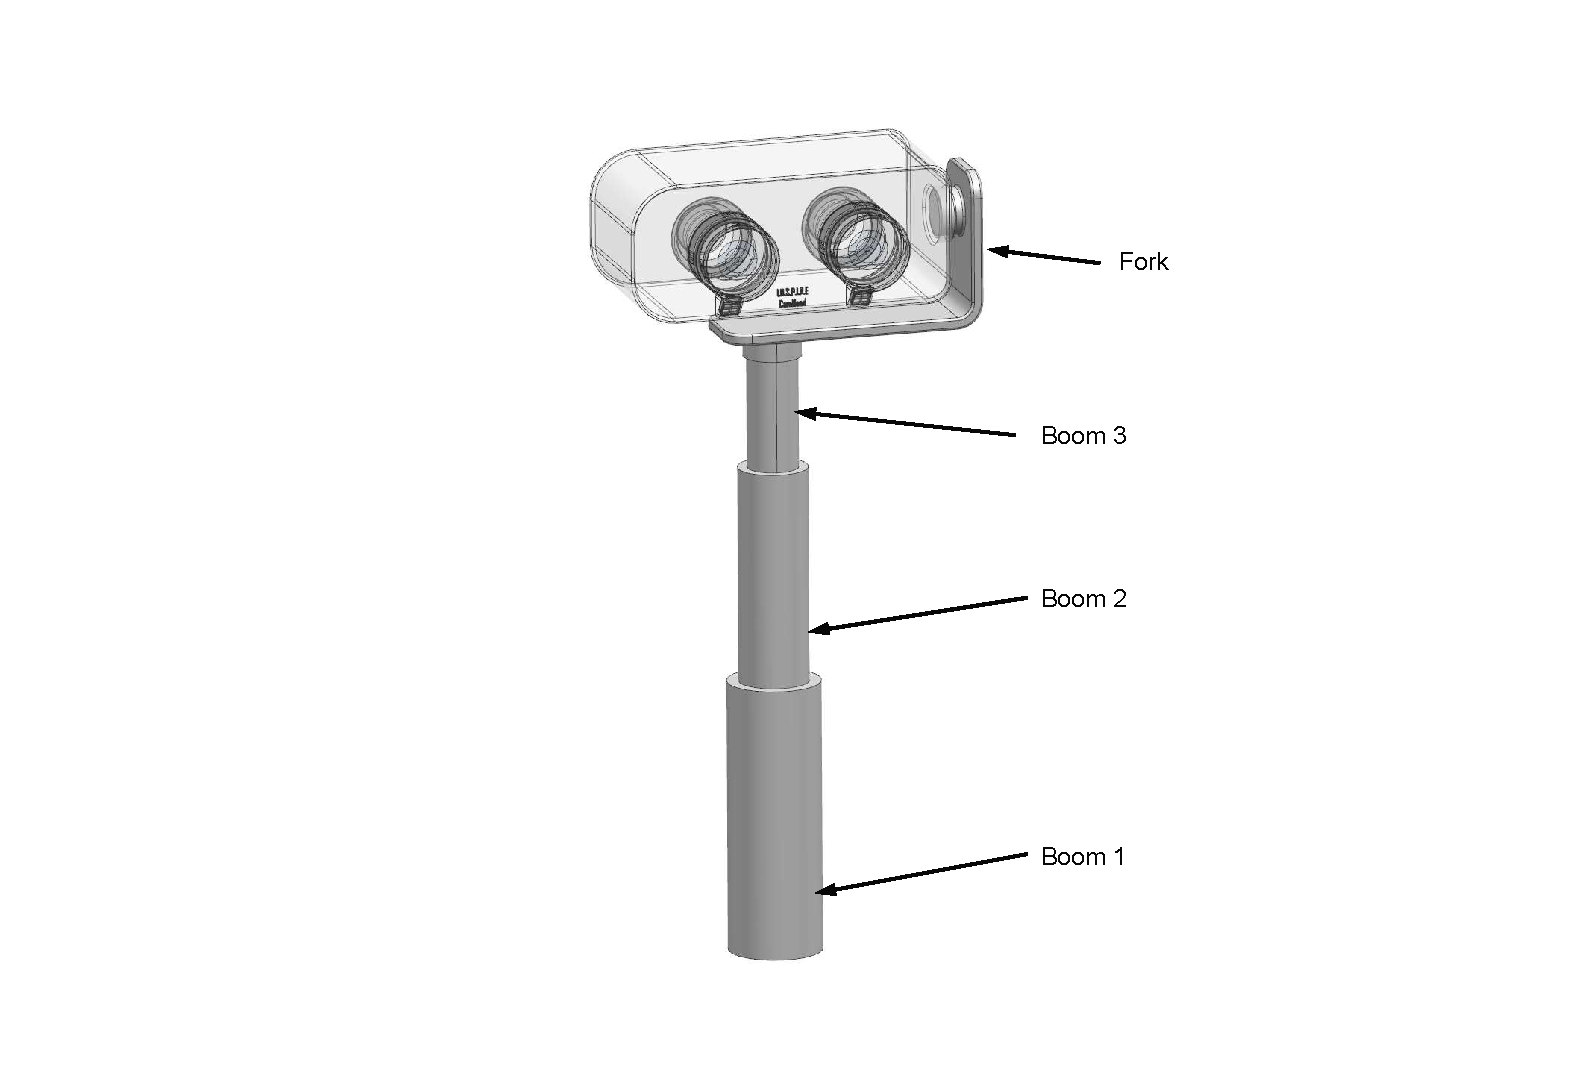
\includegraphics[width=0.25\textwidth]{Media/tcs_con_boom}}}}  \\[1em]
		& & & &  \\
		\multicolumn{2}{l}{$CON_6= \left( \frac{1}{CON_{B1}} +\frac{1}{CON_{B2}}+\frac{1}{CON_{B3}}+\frac{1}{CON_{F}} \right)^{-1} $} & & & \\[2em]
		\multicolumn{2}{l}{$CON_6= 7.10 \cdot 10^{-2}\ \frac{\W}{\K}$} & & &  \\[8em]
		\hline
		Part &  Cross section & Length  & Material & Amount \\ \hline
		& & & & \\[-0.75em]
		Boom 1 & $S_{B1}= 181 \ \mm^2$ & $l_{B1}=116 \ \mm$ & Aluminium & 1 \\[0.5em]
		Boom 2 & $S_{B2}= 134 \ \mm^2$ & $ll_{B2}=95 \ \mm$ & Aluminium & 1 \\[0.5em]
		Boom 3 & $S_{B3}= 97 \ \mm^2$ & $l_{B3}= 60\ \mm$ & Aluminium & 1 \\[0.5em]
		Fork & $S_{F}= 200\ \mm^2$ & $l_{F}=170\ \mm$ & Aluminium & 1 \\
		\label{tab:tcs_nodes2}
	\end{tabular}
\end{table}	

\begin{table}[H]
\centering
\caption{Definition of heat conductance $CON=\frac{1}{R}$ between the nodes according to \autoref{fig:tcs_network}.}
\begin{tabular}{l@{\qquad}cccc}		
		\hline
		Name &  Linked Components &  \multicolumn{3}{c}{Geometry}\\ \hline
		& & & & \\[-0.5em]
		\textbf{Suspension} & \textbf{Chassis} $\leftrightarrow$ \textbf{Node$_1$}  &  \multicolumn{3}{c}{\multirow{2}{*}{\adjustbox{valign=t}{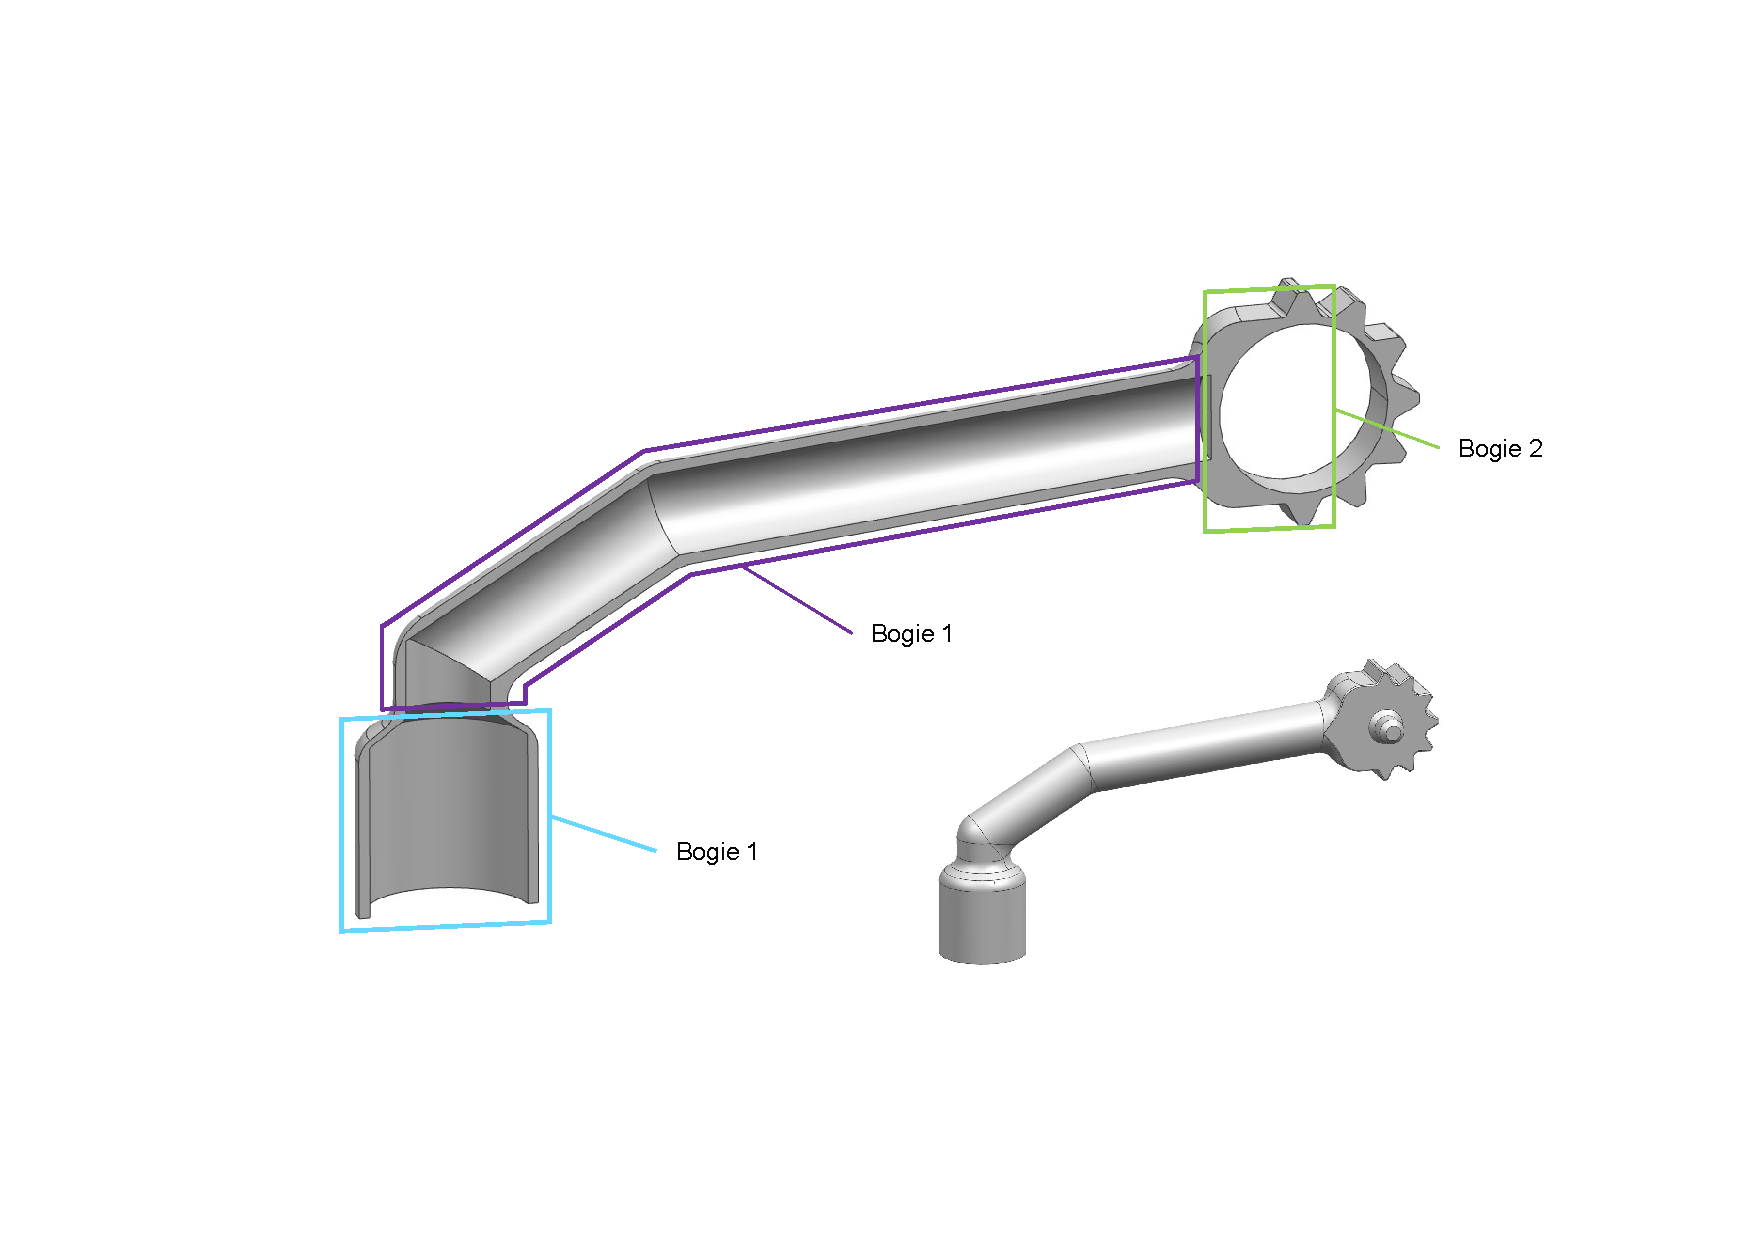
\includegraphics[width=0.455\textwidth]{Media/tcs_con_bogie}}}}  \\[1em]
		& & & &  \\
		\multicolumn{2}{l}{$CON_7=\left( \frac{1}{CON_{B1}} +\frac{1}{CON_{B2}}+\frac{1}{CON_{B3}}\right)^{-1}$} & & & \\[1em]
		\multicolumn{2}{l}{$CON_7= 1.30 \cdot 10^{-1}\ \frac{\W}{\K}$} & & & \\[6em]
		
		\hline
		Part &  Cross section & Length  & Material & Amount \\ \hline
		& & & & \\[-0.75em]
		Bogie 1 & $S_{B1}=275 \ \mm^2$ & $t_{B1}=20\ \mm$ & Aluminium & 1 \\[0.5em]
		Bogie 2 & $S_{B2}=113 \ \mm^2$ & $t_{B2}=162\ \mm$ & Aluminium & 1 \\[0.5em]
		Bogie 3 & $S_{B3}=201 \ \mm^2$ & $t_{B3}=37\ \mm$ & Aluminium & 1 \\[5em]		

		\hline
		Name &  Linked Components &  \multicolumn{3}{c}{Geometry}\\ \hline
		& & & & \\[-0.75em]
		\textbf{Mounting} & \textbf{Steer Engine} $\leftrightarrow$ \textbf{Node$_1$}  &  \multicolumn{3}{c}{\multirow{2}{*}{\adjustbox{valign=t}{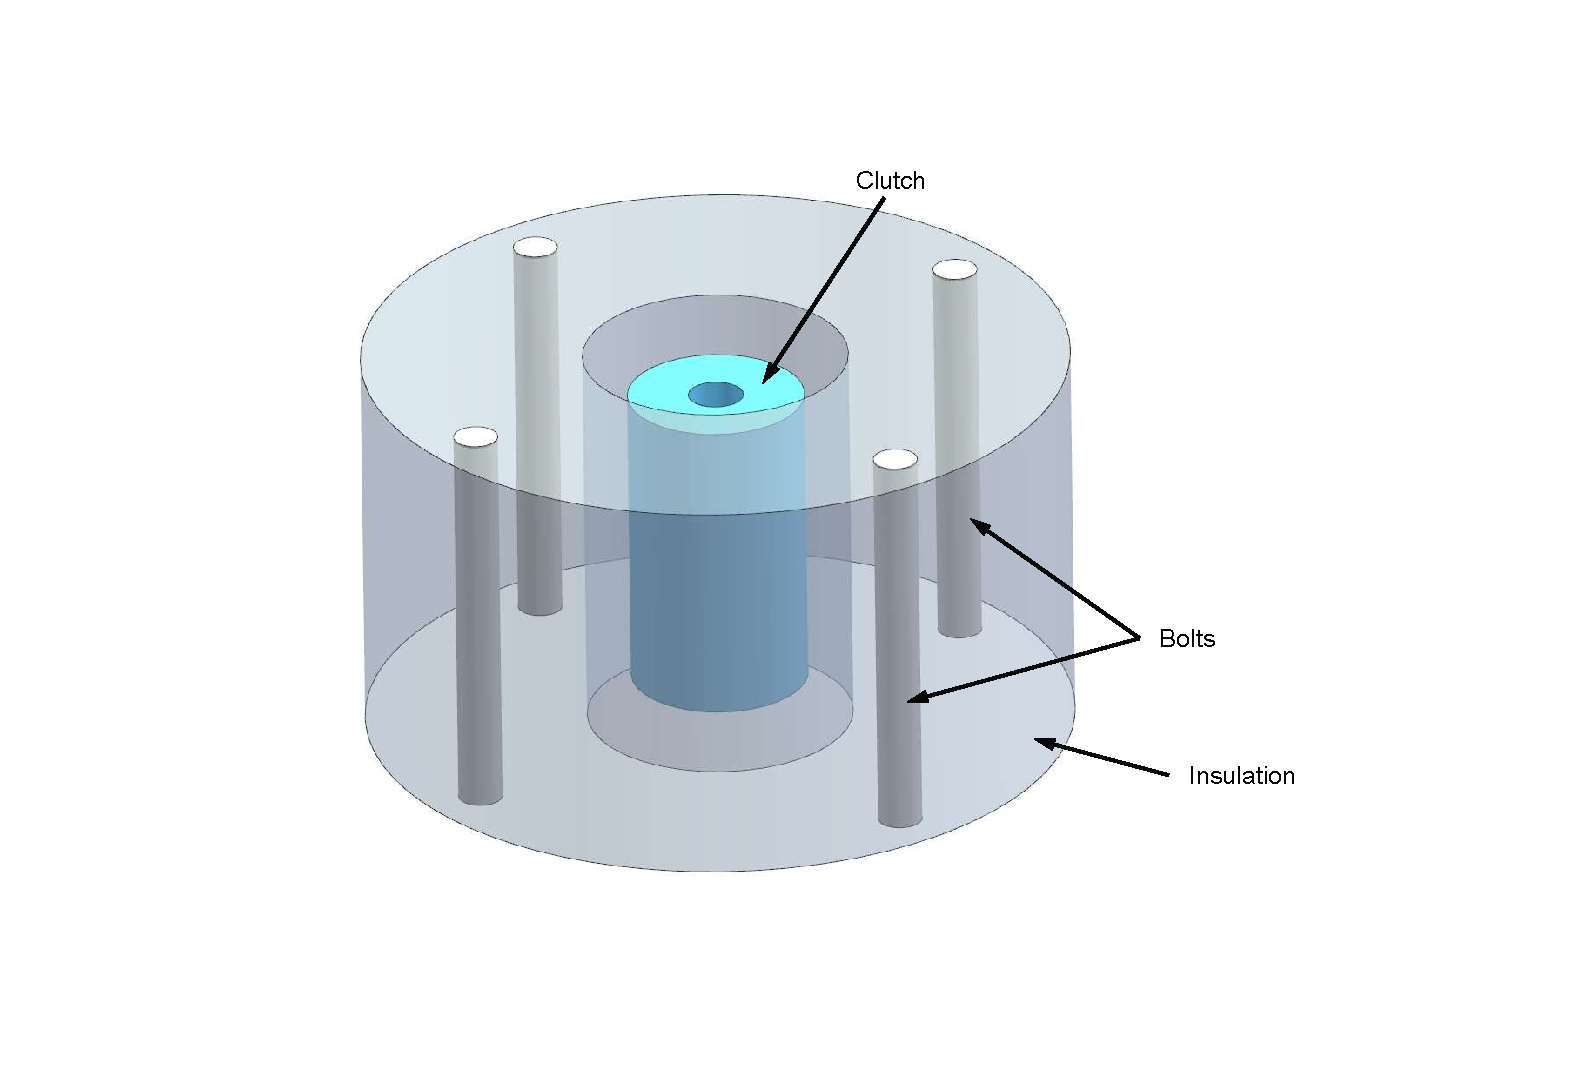
\includegraphics[width=0.4\textwidth]{Media/tcs_con_steer}}}}  \\[1em]
		& & & &  \\
		\multicolumn{2}{l}{$CON_8=CON_C+CON_I+n_B\cdot CON_B  $} & & & \\[2em]
		\multicolumn{2}{l}{$CON_8= 6.85\cdot 10^{-1}\ \frac{\W}{\K}$} & & &  \\[6em]
		\hline
		Part &  Cross section & Thickness  & Material & Amount \\ \hline
		& & & & \\[-0.75em]
		Clutch & $S_{C}= 45.4 \ \mm^2$ & $t_{C}=14 \ \mm$ & Aluminium  & 1 \\[0.5em]
		Insulation & $S_{I}= 691 \ \mm^2$ & $t_{I}=18 \ \mm$ & Aerogel & 1 \\[0.5em]
		Bolts & $S_{B}= 3.14 \ \mm^2$ & $t_{B}= 18\ \mm$ & Steel & 4 \\
		\hline
		\label{tab:tcs_nodes3}
	\end{tabular}
\end{table}	


\begin{table}[H]
	\centering
	\caption{Definition of heat conductance $CON=\frac{1}{R}$ between the nodes according to \autoref{fig:tcs_network}.}
	\begin{tabular}{l@{\qquad}cccc}		
		Name &  Linked Components &  \multicolumn{3}{c}{Geometry}\\ \hline
		& & & & \\[-0.5em]
		\textbf{Wheel Fork} & \textbf{Node$_1$} $\leftrightarrow$ \textbf{Node$_2$}  &  \multicolumn{3}{c}{\multirow{2}{*}{\adjustbox{valign=t}{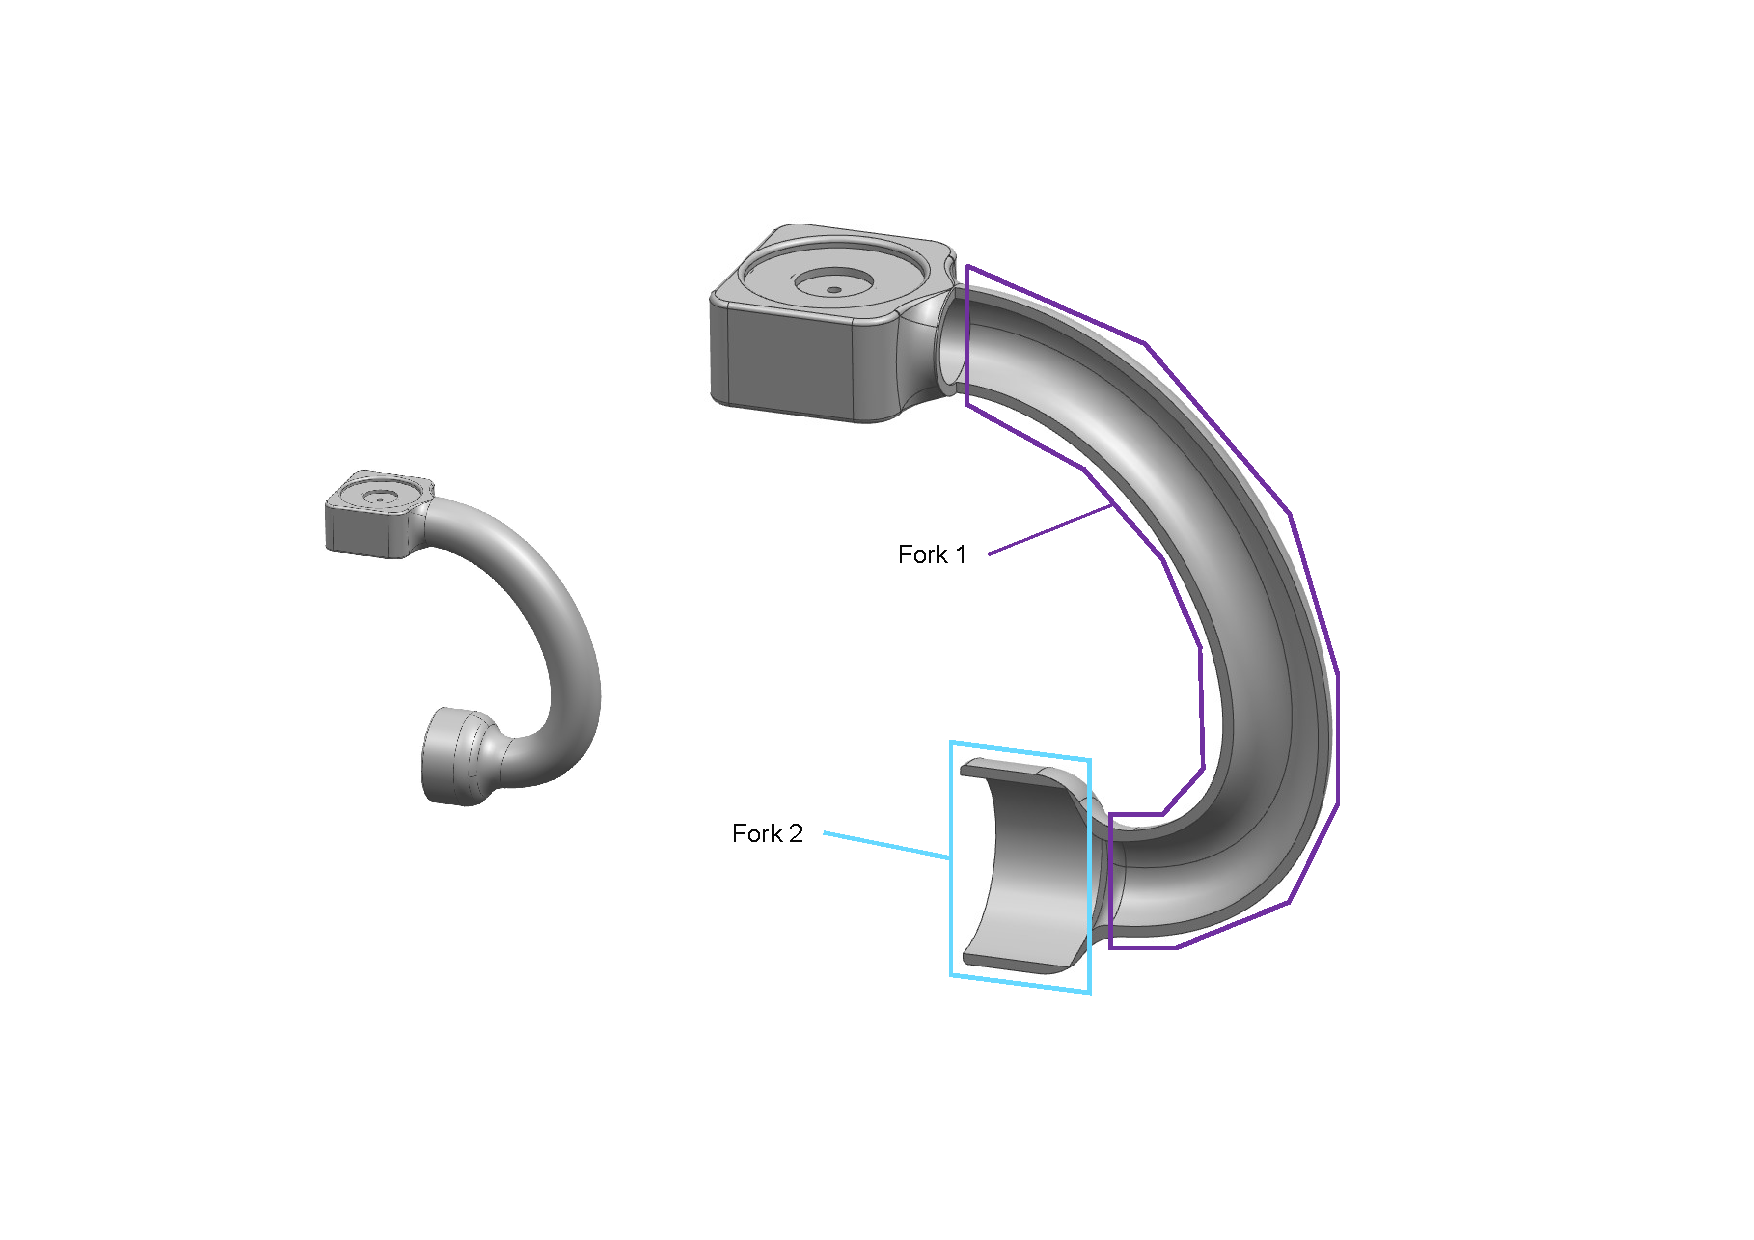
\includegraphics[width=0.45\textwidth]{Media/tcs_con_fork}}}}  \\[1em]
		& & & &  \\
		\multicolumn{2}{l}{$CON_{10}=\left( \frac{1}{CON_{F1}} +\frac{1}{CON_{F2}}\right)^{-1} $} & & & \\[1em]
		\multicolumn{2}{l}{$CON_{10}= 1.46 \cdot 10^{-1}\ \frac{\W}{\K}$} & & & \\[8em]
		
		\hline
		Part &  Cross section & Length  & Material & Amount \\ \hline
		& & & & \\[-0.75em]
		Fork 1& $S_{F1}=200 \ \mm^2$ & $l_{F1}=175$ & Aluminium & 1 \\[0.5em]	
		Fork 1& $S_{F2}=200 \ \mm^2$ & $l_{F2}=175$ & Aluminium & 1 \\[5em]	

		\hline
		Name &  Linked Components &  \multicolumn{3}{c}{Geometry}\\ \hline
		& & & & \\[-0.5em]
		\textbf{Mounting} & \textbf{Drive Engine} $\leftrightarrow$ \textbf{Node$_2$}  &  \multicolumn{3}{c}{\multirow{2}{*}{\adjustbox{valign=t}{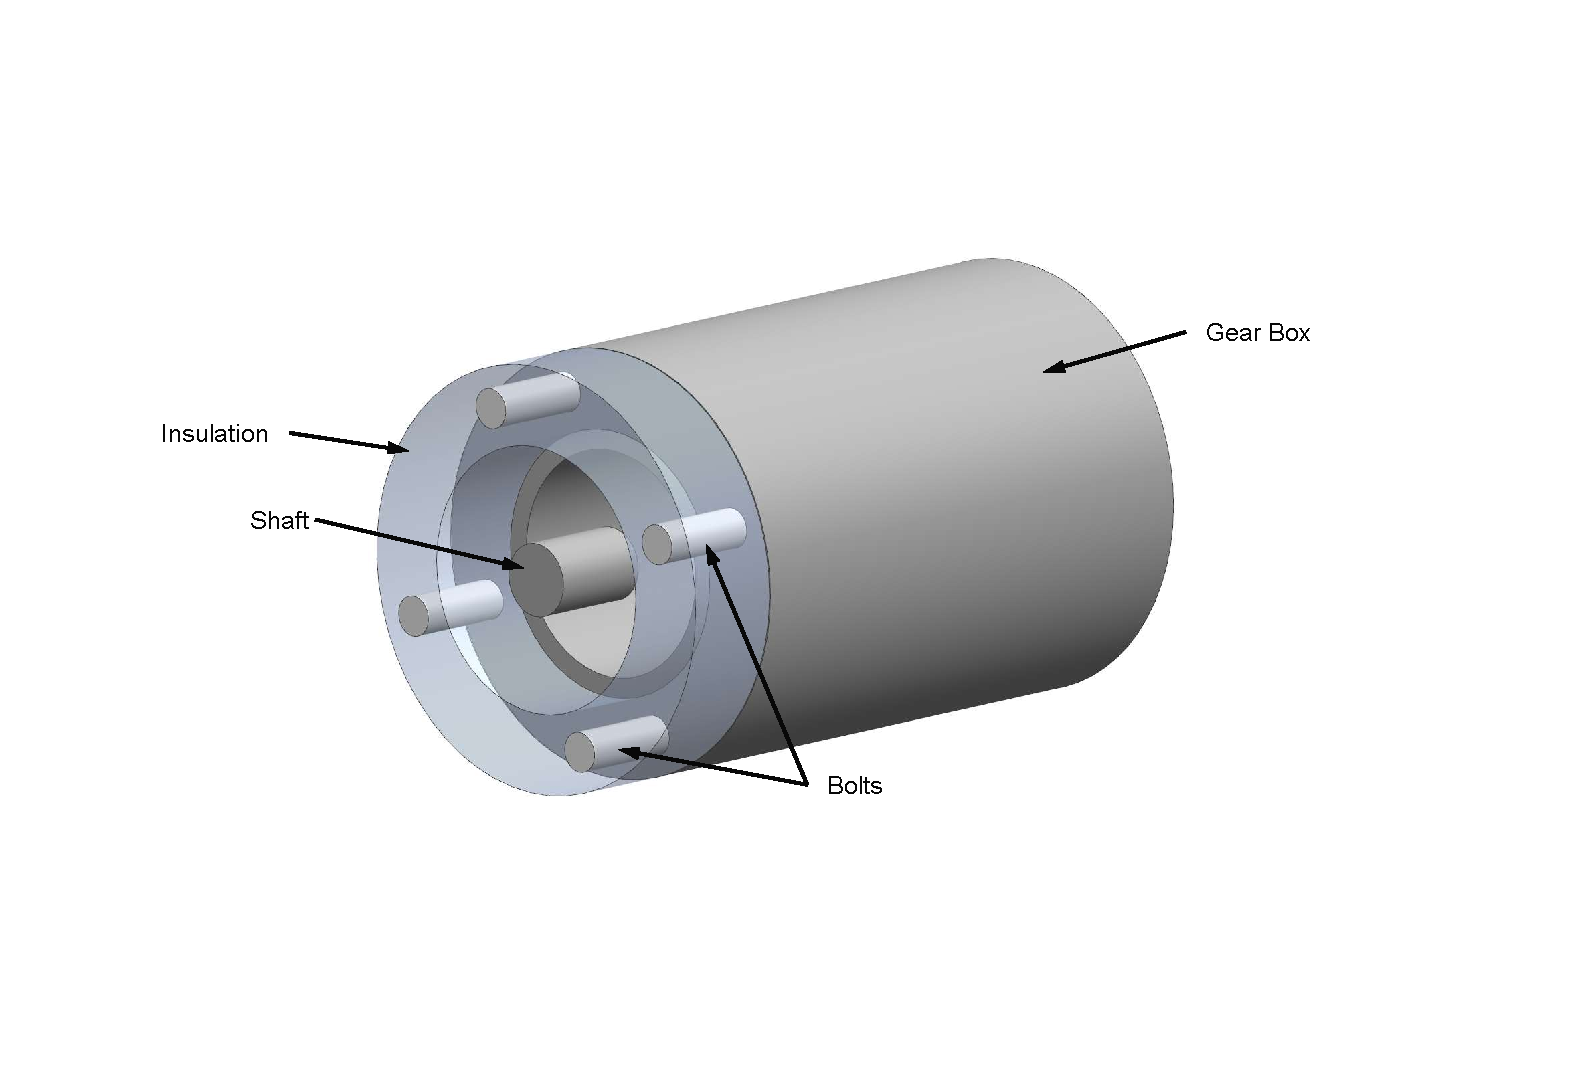
\includegraphics[width=0.5\textwidth]{Media/tcs_con_drive}}}}  \\[1em]
		& & & &  \\
		\multicolumn{2}{l}{$CON_{11}=  \left( \frac{1}{CON_G} +\frac{1}{CON_S+CON_I+n_B\cdot CON_B} \right)^{-1} $} & & & \\[2em]
		\multicolumn{2}{l}{$CON_{11}= 2.19 \cdot 10^{-1}\ \frac{\W}{\K}$} & & & \\[5em]
		
		\hline
		Part &  Cross section & Thickness  & Material & Amount \\ \hline
		& & & & \\[-0.75em]
		Gear Box & $S_{G}= 566 \ \mm^2$ & $t_{G}= 43.1\ \mm$ & Steel & 1 \\[0.5em]
		Shaft & $S_{S}= 23.8 \ \mm^2$ & $t_{S}=8 \ \mm$ & Steel & 1 \\[0.5em]
		Insulation & $S_{I}=490  \ \mm^2$ & $t_{I}=8 \ \mm$ & Aerogel  & 1 \\[0.5em]
		Bolts, M3 & $S_{B}=7.07  \ \mm^2$ & $t_{B}= 8\ \mm$ & Steel  & 4 \\[5em]	
	\end{tabular}
\label{tab:tcs_nodes4}
\end{table}	


\begin{table}[H]
	\centering
	\caption{Definition of heat conductance $CON=\frac{1}{R}$ between the nodes according to \autoref{fig:tcs_network}.}
	\begin{tabular}{l@{\qquad}cccc}		
		\hline
		Name &  Linked Components &  \multicolumn{3}{c}{Geometry}\\ \hline
		& & & & \\[-0.5em]
		\textbf{Rim} & \textbf{Node$_2$} $\leftrightarrow$ \textbf{Ground}  &  \multicolumn{3}{c}{\multirow{2}{*}{\adjustbox{valign=t}{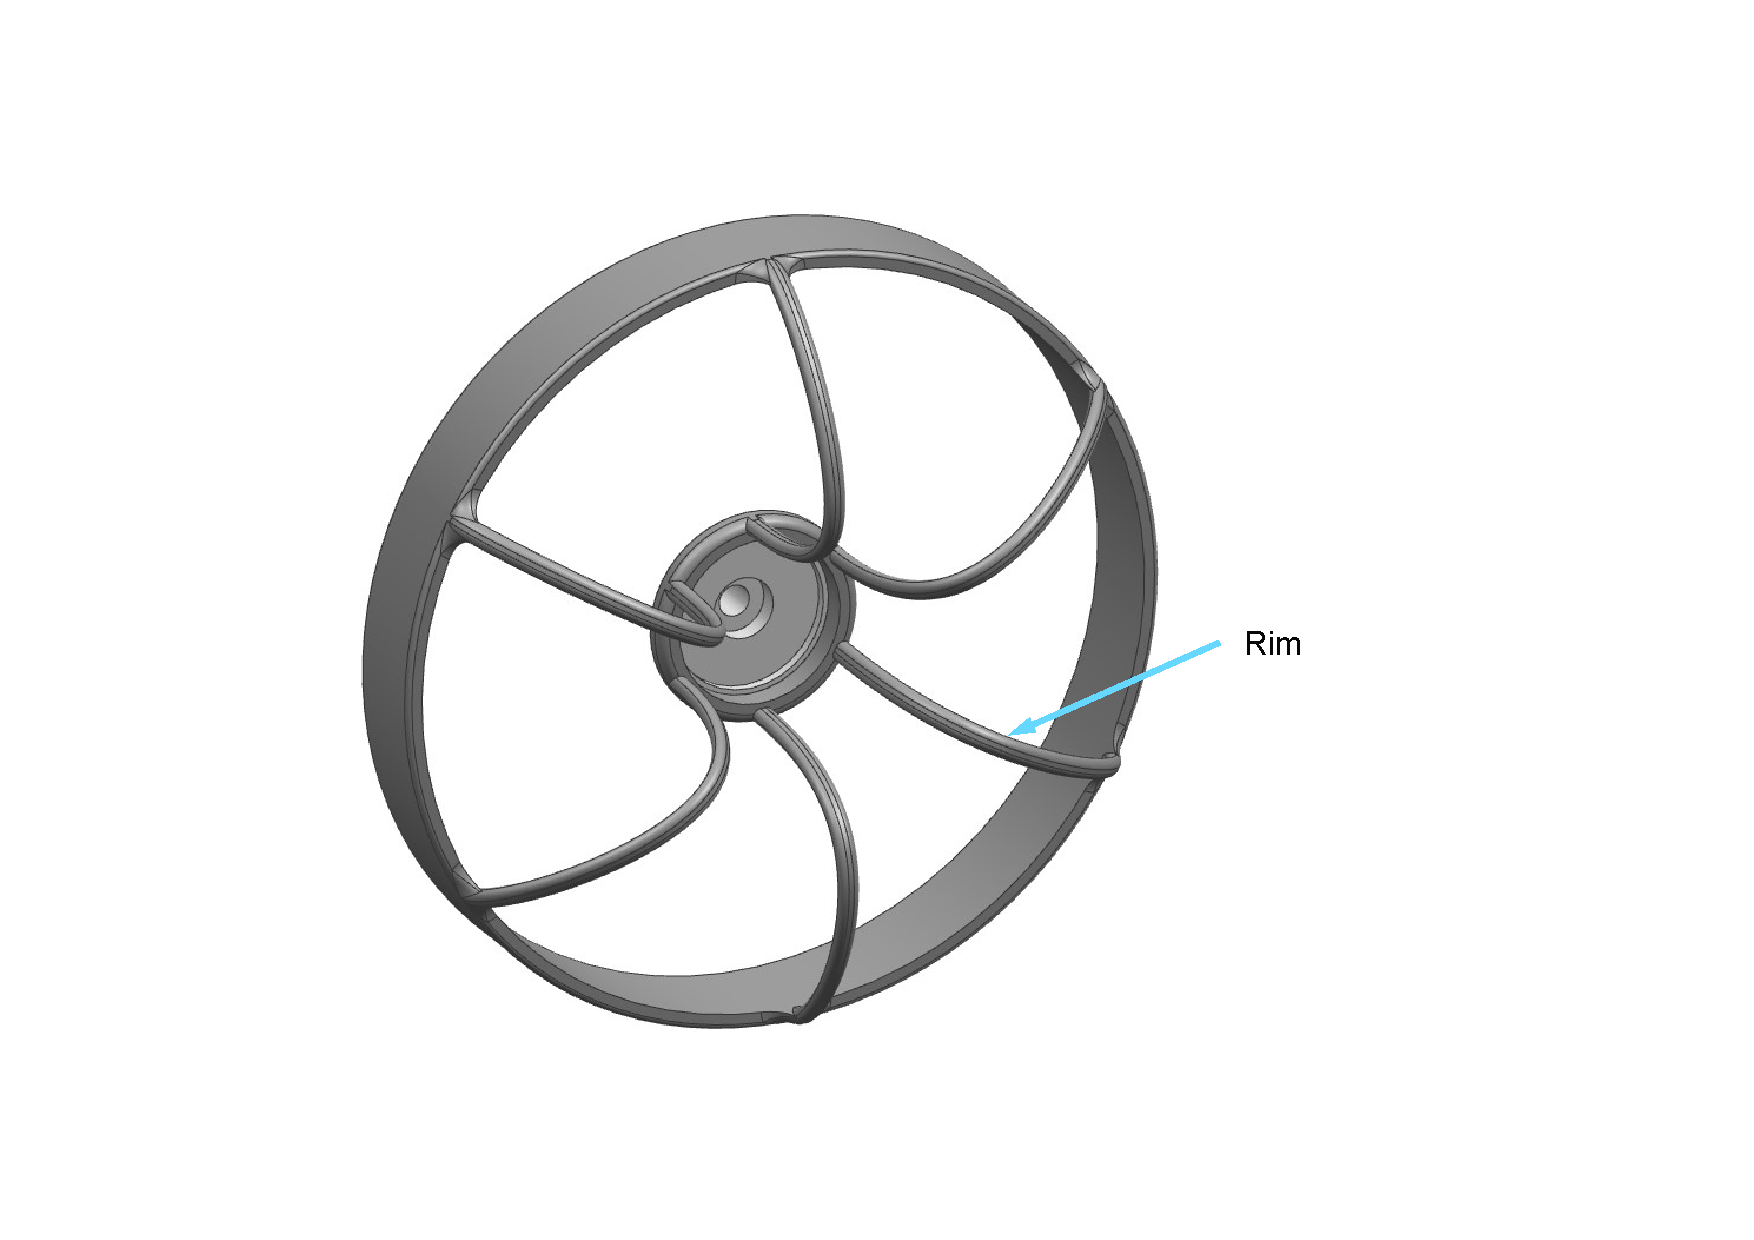
\includegraphics[width=0.3\textwidth]{Media/tcs_con_rim}}}}  \\[1em]
		& & & &  \\
		\multicolumn{2}{l}{$CON_{13}= 5.11 \cdot 10^{-3}\ \frac{\W}{\K}$} & & & \\[7em]
		
		\hline
		Part &  Cross section & Length  & Material & Amount \\ \hline
		& & & & \\[-0.75em]
		Rim & $S_R=12 \ \mm^2$ & $l_r=100\ \mm$ & Aluminium & 6 \\[1.5em]
		\multicolumn{5}{l}{\textit{Note}: It was assumed, that the wheel temperature equals the surface temperature} \\
		\multicolumn{5}{l}{because of the thin rims and resulting low heat conduction.} \\[3em]	
	\end{tabular}
\label{tab:tcs_nodes5}
\end{table}	

\subsection{Heat switch} \label{sec:app_therm_3}
The charateristic of the switch conductance depends on the mean temperature $T_M$, shown by measurements in cite .
As this temperature won´t be calculated in the analysis, the corresponding component temperature $T_C$ shall be used.
In order to describe the characteristic, it was diveded in three sections, \autoref{fig:tcs_switch03}.
The temperature where the disk decouples is $T_{toggle}=108 K$ and not applicable for the current application.
By reducing the heigt, the toggle temperature can be increased and the characteristic can be shifted to higher termperatures ("to the right").
It was assumed, that the gradients of section 2 and 3 as well as the temperature range of section 2 keep constant.
The axis interseption is a function the toggle temperature ($a_2=f(\Delta T_{toggle}),\ \Delta T_{Toggle}=T_{new}-T_{old}|_{toggle}$).
The used toggle temperature are listed in autoref
\begin{table}[H]
	\centering
	\caption{Sections and range of the switch characteristic.}
	\begin{tabular}{c@{\qquad}rcl@{\qquad}l}
		\hline
		Section & \multicolumn{3}{l}{Temperature range} & Heat conductance $CON_S= \frac{1}{R_t}$ \\ \hline
		& & & &  \\[-0.5em]
		1 & $T_{toggle} >$ & $ T_C  $ & & $CON_{S}= 16.4 \cdot 10^{-3}\ \frac{\W}{\m^2 \K} = const.$\\[1.5em]
		2 & $T_{toggle}\leq$ & $ T_C $ & $ < T_1$ & $CON_{S} (T_C) = a_{1.1} \cdot T_C+ a_{1.2}$\\[1em]
		& & & & $a_{1.1}= +1.272\cdot 10^{-3}\ \frac{\W}{\m^2 \K^2}$ \\[1em]
		& & & & $  a_{1.2}= -1.272\cdot 10^{-3}\ \frac{\W}{\m^2 \K^2}\cdot \Delta T_{Toggle}-0.117\ \frac{\W}{\m^2 \K}$  \\[2em]
		3 & & 	$ T_C$ & $^ > T_1$ & $CON_{S}(T_C) = a_{2.1} \cdot T_C+ a_{2.2}$\\[1em]
		& & & & $a_{2.1}=+ 333\cdot 10^{-6}\ \frac{\W}{\m^2 \K^2}$ \\[1em]
		& & & & $  a_{2.2}= -333\cdot 10^{-6}\ \frac{\W}{\m^2 \K^2}\cdot \Delta T_{Toggle}-28.3 \cdot 10^{-3}\ \frac{\W}{\m^2 \K}$  \\[1em] \hline
	\end{tabular}
	\label{tab:tcs_section}
\end{table}

\begin{figure}[H]
	\centering
	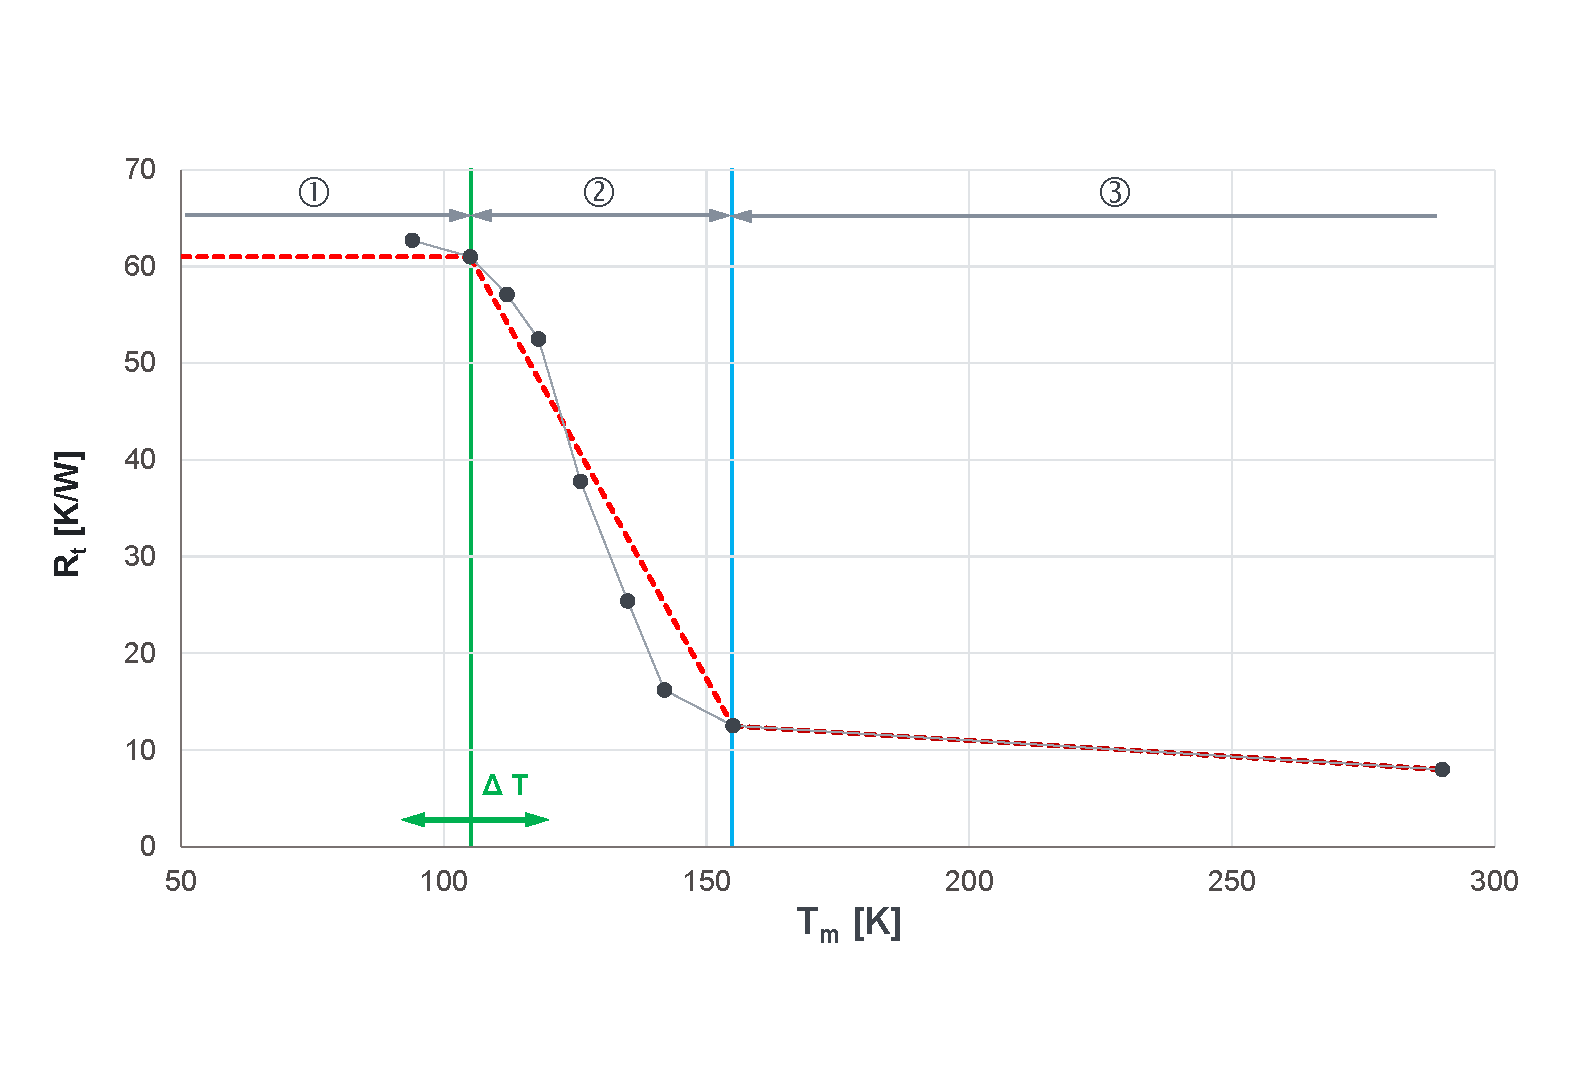
\includegraphics[width=1\textwidth]{Media/tcs_diag_section}
	\caption{Conductance characteristic of heat switch diveded in sections.}
	\label{fig:tcs_switch03}
\end{figure}


\begin{table}[H]
	\centering
	\caption{Toggle temperature and amount of bi-metallic heat switch.}
	\begin{tabular}{c@{\quad}ccc}
		\hline
		Heat switch name  & Linked Components & Temperature  & Amount \\ \hline
		$CON_{S1}$ & {Camera} $\leftrightarrow$ {Radiator} & -20\ $^\circ$C  & $n_{S1}=$4  \\[1em]
		$CON_{S2}$ & {EBay} $\leftrightarrow$ {Chassis} & -30\ $^\circ$C  & $n_{S2}=$2  \\[1em]
		$CON_{S3}$ & {Drive Engine} $\leftrightarrow$ {Node$_2$} & -20\ $^\circ$C  & $n_{S3}=1$  \\
	 			&											&						& (in total 4)  \\\hline
	\end{tabular}
	\label{tab:tcs_toggle}
\end{table}

\subsection{Rover absorptivity} \label{sec:app_therm_4}
The rover position relativ to the direct sun radiation is given by the ecliptic longitude $\lambda_R$ and latitude $\delta_R$ angle, where the axis $x_E$ points always to the sun, \autoref{fig:tcs_rad2}.
The amount of solar radiation $S_0$ absorbed by the rover surfaces depends on the sun altitude and can be determined by the view factor $\varphi$, see \autoref{fig:tcs_rad1}.
The view factors during eclipse are set to zero.

\begin{table}[H]
	\begin{tabular}{l@{\qquad}ll}
		View Factor 1,& horizontal surface:& $ \varphi_1=\cos (\lambda_R) \cdot \cos (\delta_R)  $ \\
		View Factor 2, & vertical surface: &$ \varphi_2=\cos (90^{\circ}-\lambda_R) \cdot \cos (\delta_R)  $\\
	\end{tabular}
\end{table}

\begin{figure}[h]
	\centering
	\subfloat[View factor depending on the absorbtion surface.]{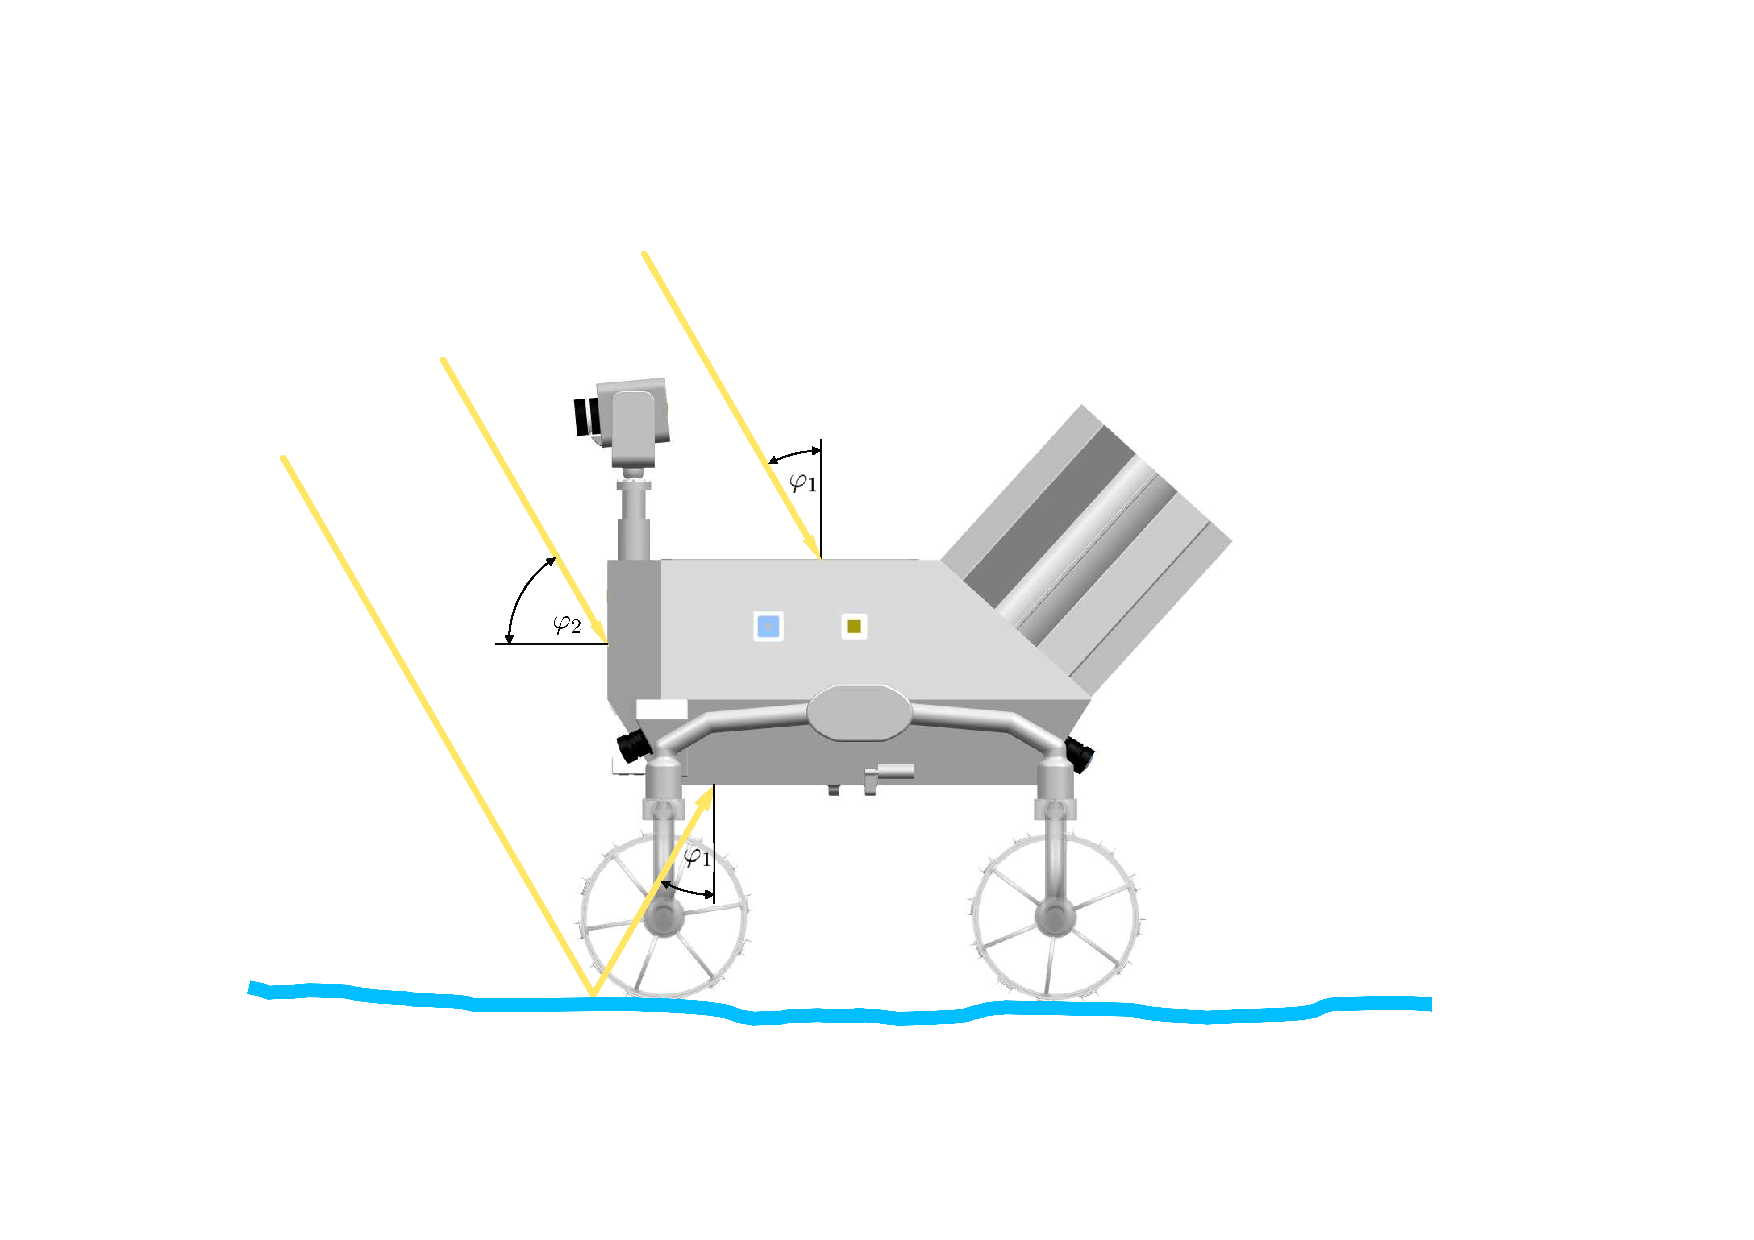
\includegraphics[height=0.4\textwidth]{Media/tcs_rover_rad}\label{fig:tcs_rad1}}\qquad\qquad
	\subfloat[Definition of ecliptic longitude $\lambda_R$ and latitude $\delta_R$ of the rover on Europa.]{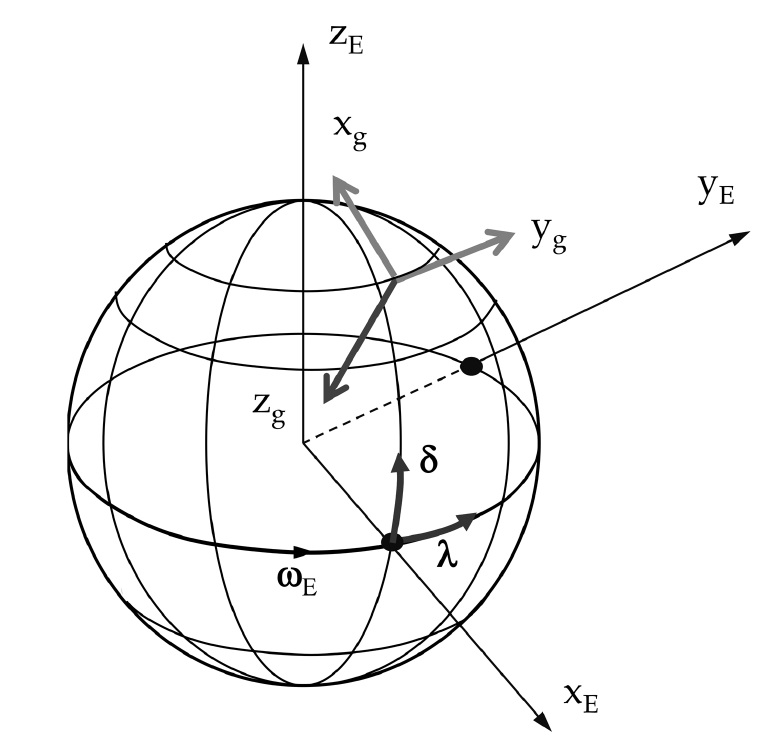
\includegraphics[height=0.3\textwidth]{Media/tcs_angle.png}\label{fig:tcs_rad2}}
	\caption{Bi-metallic heat switch, \cite{ref_tcs_04}.}
	\label{fig:tcs_rad}
\end{figure}


\subsection{Input Values} \label{sec:app_therm_5}
\begin{table}[H]
	\centering
	\caption{Temperatur limits of the rover components.}
	\begin{tabular}{lccc}
		\hline 
		& \multicolumn{2}{l}{Temperature limits in [$^\circ$C]} & Source\\ 
		Component	&	min. & max. &\\\hline
		OBC & -55 & 70 & \\
		Transmitter & -10 & 50 & \\
		Receiver & -30 & 70 & \\
		PCDU & -40 & 60 & \\
		Battery & -20 & 60 & \cite{SAFTBatteries.2018}\\
		Camera & -40 & 70  & \\
		Objektive  & -40 & 71 & \\
		Steering Engine & -30 & 100 & \\
		Drive Engine & -40 & 100 & \\
		Drive Gear & -40 & 100  & \\ \hline
	\end{tabular}
	\label{tab:tcs_limits}
\end{table}

\begin{figure}[H] 
	\centering
	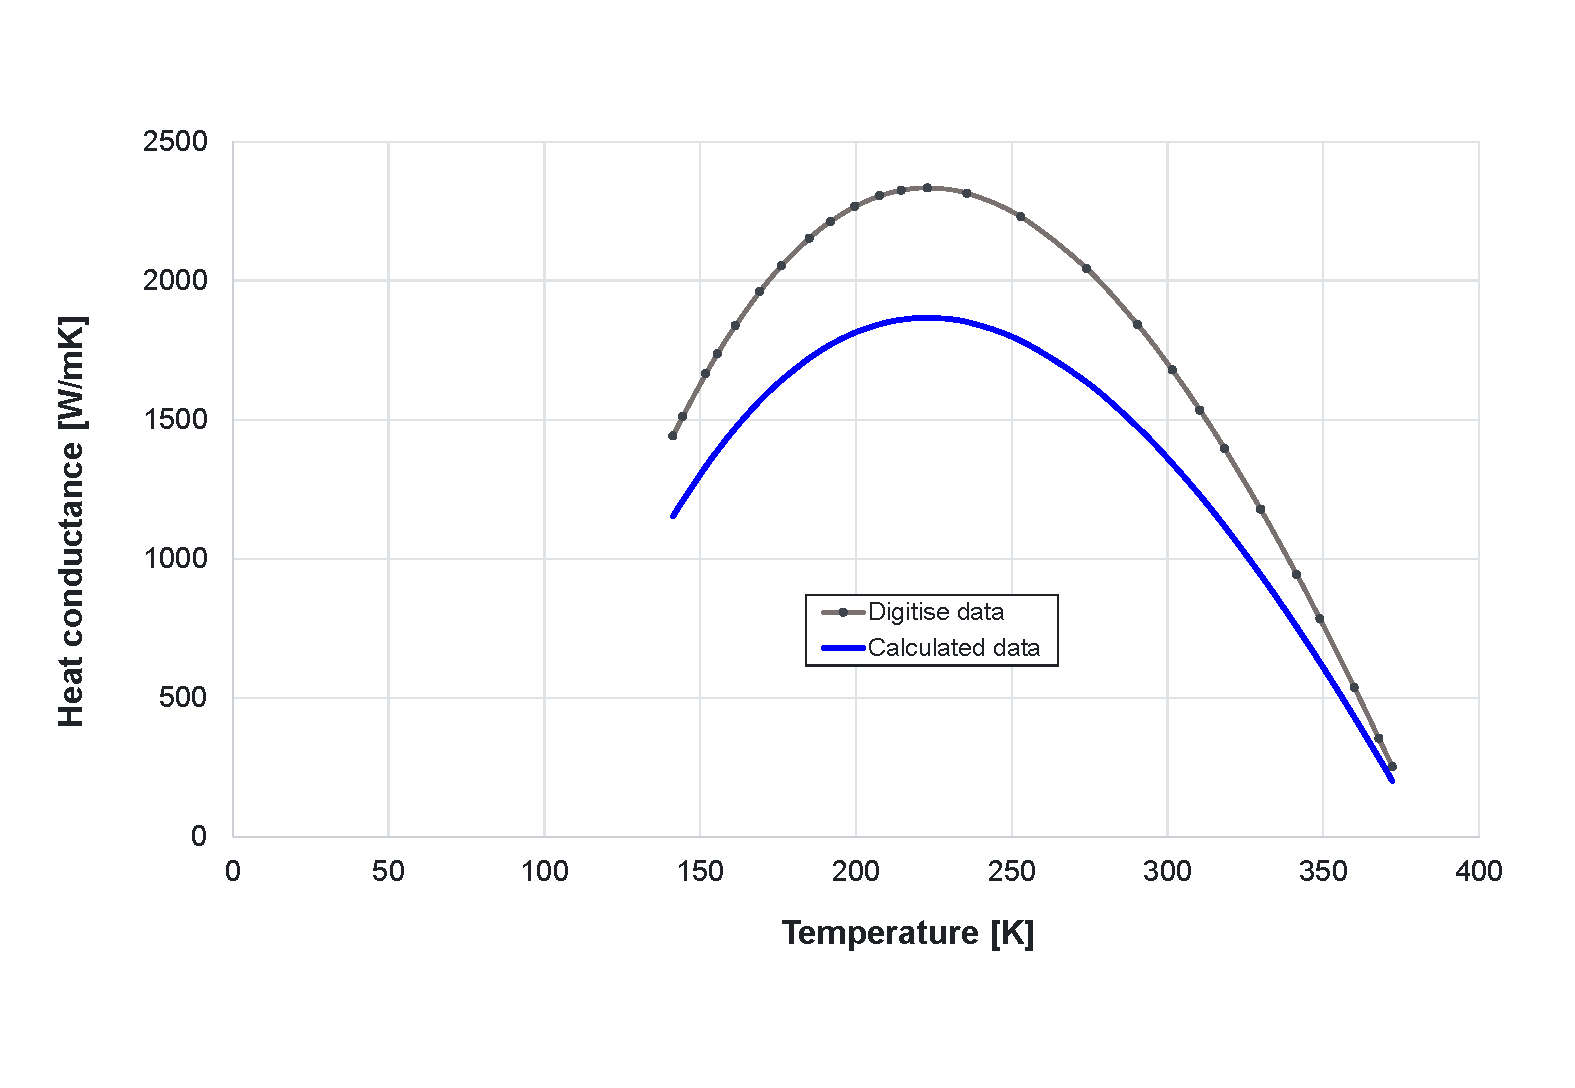
\includegraphics[width=0.8\textwidth]{Media/tcs_lynx_calc}
	\caption{Digitalised \cite{ref_tcs_01} and calculated heat conduction in comparison.}
	\label{fig:tcs_lynx}
\end{figure}
The characteristic of the \textit{LyNX}\textsuperscript{\tiny\textregistered} conduction was approximated with follwing function,
\begin{equation}
\lambda(T)= \left(1.76 \cdot 10^{-4}\ \frac{\W}{\m \K^4} \cdot T^3 -2.37\cdot 10^{-1}\ \frac{\W}{\m \K^3} \cdot T^2 +79.5 \frac{\W}{\m \K^2} \cdot T -5.55\cdot 10^{3}\ \frac{\W}{\m \K}\right) \cdot f_{r}  
\label{eq:tcs_lynx}
\end{equation}
with the reduction fator $f_{r}$=0.8.

\begin{table}[H]
	\centering
	\caption{Dimensions of the thermal straps \textit{LyNX}\textsuperscript{\tiny\textregistered}.}
	\begin{tabular}{l@{\quad}cc}
		\hline
		Linked Components & Cross section  & Length$^{1)}$  \\ \hline
		EBay $\leftrightarrow$ RTG & 42\ mm$^2$ & 230 mm  \\[0.25em] 
		Drill $\leftrightarrow$ RTG &10 \ mm$^2$ &345 \ mm \\[0.25em] 
		Steer Engine $\leftrightarrow$ RTG & 36\ mm$^2$&644\ mm  \\[0.25em] 
		Drive Engine $\leftrightarrow$ RTG &42 \ mm$^2$&897\ mm  \\[0.25em] \hline
		& &   \\[-0.5em]
		\multicolumn{3}{l}{$^{1)}$\ Du to uncertainties the length was increased about 15\%.}\\[1em]
	\end{tabular}
	\label{tab:tcs_lynx}
\end{table}

The Europa surface temperature varies at the  equator between $T_{e,min}=80$\ K and\\ $T_{e,max}=130$\ K, depending on the sun inclination.
The temperature at the pole is $T_{Pole}=50$\ K, \cite{Europa}.
It was assumed, that the surface temperature depends on the sun altitude.
A trigonometrical interpolation was defined as follows.
\[ T_{Surface}(\lambda, \delta) = T_{Pole} + \cos (\delta) \cdot [(T_{e,min}+\cos (\lambda)\cdot (T_{e,max}-T_{e,min}))-T_{Pole}] \]
For $\lambda$ and $\delta$ see \autoref{sec:app_therm_4}.\\

\begin{table}[H]
	\centering
	\caption{Minimum and maximum of surface emisivity and absorptivity values, \cite{ref_tcs_05}.}
	\begin{tabular}{l@{\qquad\qquad}cc@{\qquad\qquad}cc}
		\hline
		& \multicolumn{2}{l}{Emisivity [-]} & \multicolumn{2}{l}{Absorptivity [-]}  \\ 
		Surface finishing	&	min. & max. 	&	min. & max.   \\\hline
		Aluminium, polished & \multicolumn{2}{c}{0.05} & \multicolumn{2}{c}{0.2}   \\
		Aluminium, sand blasted & \multicolumn{2}{c}{0.2} & \multicolumn{2}{c}{0.4}   \\
		White paint & 0.8 & 0.9 & 0.2 & 0.5  \\ \hline
		& & & & \\
	\end{tabular}
	\label{tab:tcs_surface}
\end{table}


\begin{table}[H]
	\centering
	\caption{Heat conductivity in $\frac{\W}{\m \K}$}
	\begin{tabular}{l@{\qquad\qquad}c@{\qquad\qquad}c@{\qquad\qquad}l}
		\hline
		Material & Nominal & Used & Source \\ \hline
		Aerogel & 0.002 - 0.05 & 0.05 & \cite{ref_tcs_03} \\
		Aluminium$^{1)}$  & 110 - 220 & 220 & \cite{ref_tcs_10}, \cite{ref_tcs_11}, \cite{ref_tcs_12} \\
		Steel$^{1)}$ & 15 - 43 & 45 & \cite{ref_tcs_08}, \cite{ref_tcs_09} \\ 
		Titan  & 7.1  & 7.1 & \cite{ref_tcs_06}, \cite{ref_tcs_07} \\\hline
		&&&\\[-0.75em]
		\multicolumn{4}{l}{\small{$^{1)}$\  Depends on the alloying component, a conservative value was choosen.}}\\
	\end{tabular}
	\label{tab:tcs_conduct2}
\end{table}

\begin{table}[H]
	\centering
	\caption{Radiation surface and finishing of components.}
	\begin{tabular}{l@{\qquad}l@{\qquad}ll}
		\hline
		Part  & Surface [$\m^2$] & Finishing & Note \\ \hline
		Chassis - top/bottom & $S_{Ch1}=0.086$ &  white paint & for albedo\\
		Chassis - side & $S_{Ch2}=0.081$ &  white paint & for albedo\\
		Chassis - total & $S_{Ch3}=0.423$ &  white paint & for emisivity\\
		RTG& $S_{RTG}=0.086$ & white paint & konstant emisivity of 0.9\\
		Electric Bay& $S_{Bay}=0.146$ & aluminium, sand blastet & \\
		Camera - housing & $S_{Cam}=0.027$ &aluminium, sand blastet &\\
		Camera - radiator & $S_{Rad}=0.066$ & white paint &  \\
		Steer Engine& $S_{E,S}=0.002$ & white paint& \\
		Drive Engine& $S_{E,D}=0.003$ &white paint & \\
		Bogie & $S_{B}=0.018$ &white paint & \\
		Wheel Fork& $S_{F}=0.008$ &white paint & \\ \hline
		&&& \\
		\multicolumn{3}{l}{The cross sections were taken form the CAD model.}
	\end{tabular}
	\label{tab:tcs_surf}
\end{table}

\clearpage

\setcounter{figure}{0}
\setcounter{table}{0}

\section{Radiation}

\label{sec:AppendixRadiation}

In this chapter, detailed calculations are performed on which \autoref{sec:Radiation} is based on. All calculations and figures in \autoref{sec:AppendixRadiation} are performed with SPENVIS unless otherwise stated. In order to simulate the radiation on Europa an orbit around Jupiter is simulated with the orbit parameters of Europa with a total mission duration of 30 days. The chosen parameters were an perijove altitude of 664,862 km, an apojove altitude of 676,938 km, and an inclination of 0.47°.

\subsection{Jupiters Radiation Environment}

\label{subsec:AppendixRadiationEnvironment}

In order to compare the radiation environment around Jupiter and the radiation environment around Earth the following trapped radiation models were used: for Jupiter the D\&G83+Salammbo proton model and D\&G83+GIRE+SalammboE electron model was used; for Earth the AP-8 proton model and the AE-8 electron model was used.

\begin{figure}[htb]
     \centering
     \begin{subfigure}[b]{0.49\textwidth}
         \centering
         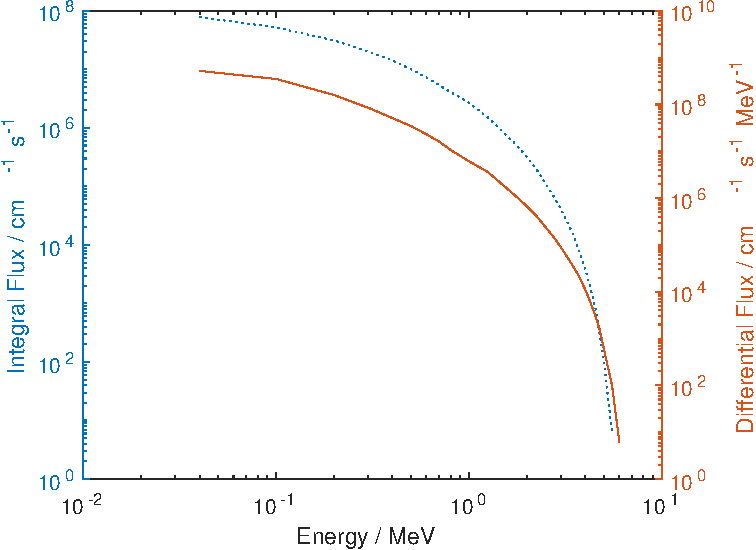
\includegraphics[width=\textwidth]{Media/E_Electron_Flux}
         \caption{Average spectra of trapped electrons around Earth}
         \label{fig:trappedelectronsEarth}
     \end{subfigure}
     \hfill
     \begin{subfigure}[b]{0.49\textwidth}
         \centering
         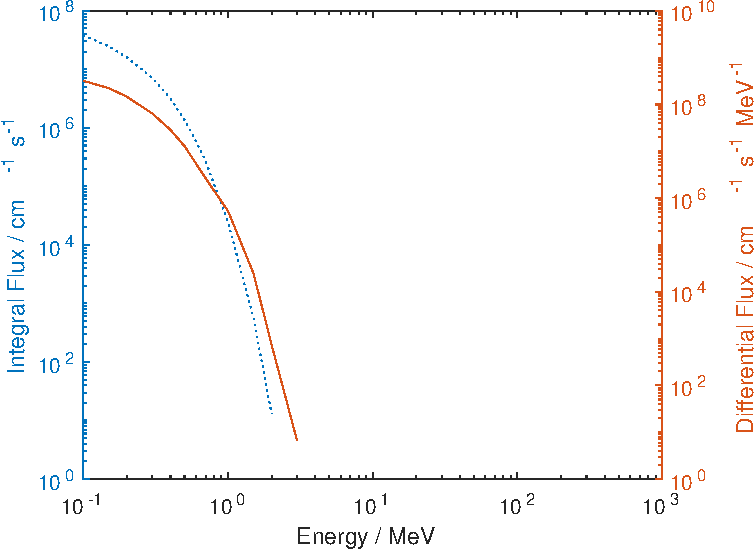
\includegraphics[width=\textwidth]{Media/E_Proton_Flux}
         \caption{Average spectra of trapped protons around Earth}
         \label{fig:trappedprotonsEarth}
     \end{subfigure}
     \hfill
     \begin{subfigure}[b]{0.49\textwidth}
         \centering
         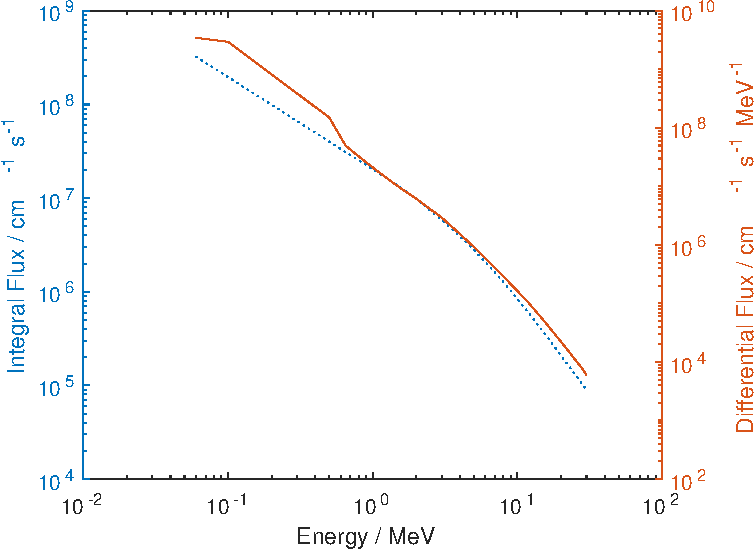
\includegraphics[width=\textwidth]{Media/J_Electron_Flux}
         \caption{Average spectra of trapped electrons around Jupiter}
         \label{fig:trappedelectronsJupiter}
     \end{subfigure}
     \hfill
     \begin{subfigure}[b]{0.49\textwidth}
         \centering
         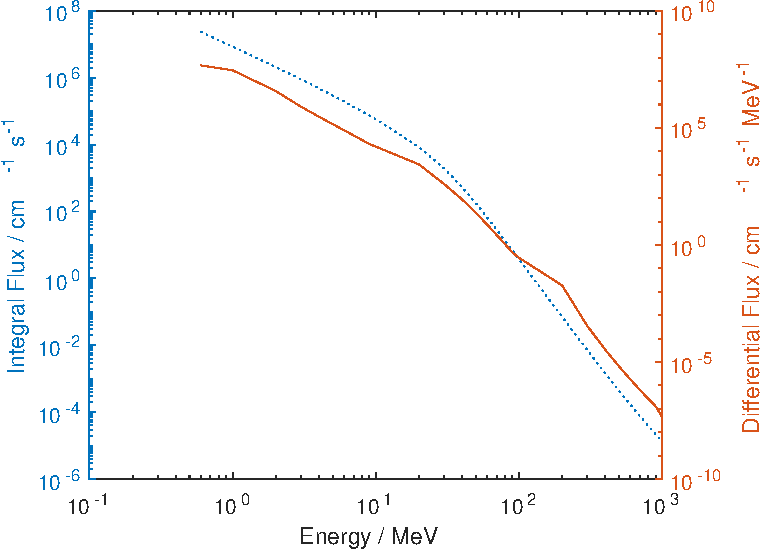
\includegraphics[width=\textwidth]{Media/J_Proton_Flux}
         \caption{Average spectra of trapped protons around Jupiter}
         \label{fig:trappedprotonsJupiter}
     \end{subfigure}
     \caption{Average trapped proton and electron fluxes on an orbit around earth at 25,000 km, through the outer Van Allen radiation belt, and on Europa's orbit around Jupiter.}
     \label{fig:trappedprotonelectronfluxes}
\end{figure}

\clearpage

\subsection{Radiation Exposures}

\label{subsec:AppendixRadiationExposures}

In order to simulate the TID for different radiation protections the Geant4 tool Multi-Layered Shielding Simulation (MULASSIS) is used. As target material silicon is selected with a thickness of 1 \(\mu \text{m}\). As shape a planar slap is selected because of the ice ground on one side of the rover.

\begin{figure}[htb]
     \centering
     \begin{subfigure}[b]{0.49\textwidth}
         \centering
         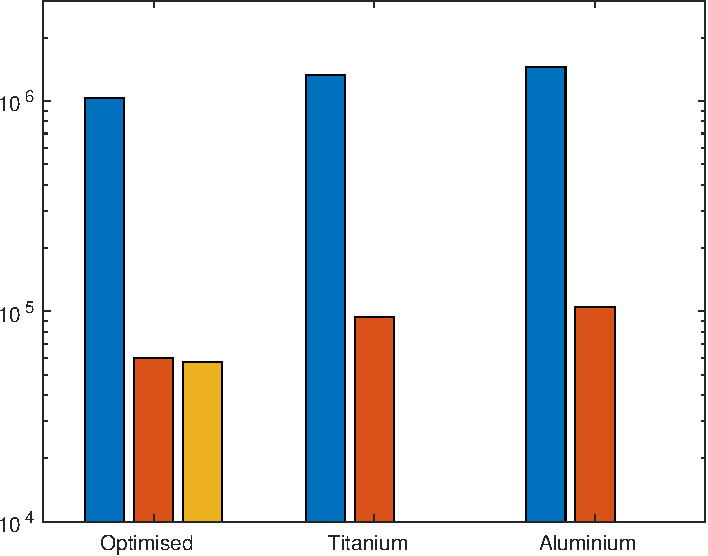
\includegraphics[width=\textwidth]{Media/J_Electron_Shielding}
         \caption{TID for Electrons as Source Particles}
         \label{fig:TIDElectronShielding}
     \end{subfigure}
     \hfill
     \begin{subfigure}[b]{0.49\textwidth}
         \centering
         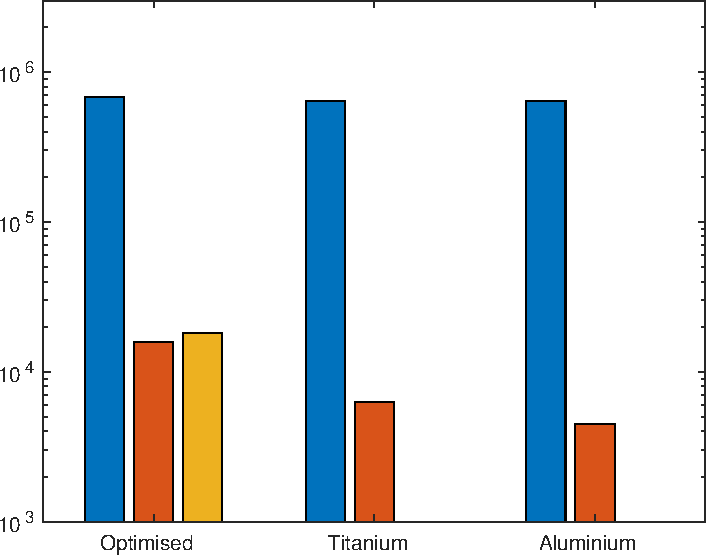
\includegraphics[width=\textwidth]{Media/J_Proton_Shielding}
         \caption{TID for Protons as Source Particles}
         \label{fig:TIDProtonShielding}
     \end{subfigure}
     \caption{TID of aluminium, titanium, and the optimised radiation structure shown in \autoref{tab:OptimalRadiationProtection} with a weight target of all three structures of 0.5 \(\text{g/cm}^2\) over 30 days of exposure on Europa.}
     \label{fig:AluminiumTitanOptimised}
\end{figure}

\begin{table}[htb]
\centering
\caption{Used components and the respective radiation tolerance and location}
\begin{adjustbox}{max width=\textwidth}
\begin{tabular}[l]{lccccc}

	\toprule
		Components	&	Rated TID	&	Exposed TID	&	Location\\
	\midrule
	
	Electric Motors	&	-	&	< 205 krad	&	locomotion housing\\	
	
	Harness	&	-	&	< 98 krad	&	chassis\\	
	
	Stereo Vision Cams	&	40	&	< 31 krad	&	camera housing\\	
	
	OBC	&	1000	&	< 17 krad	&	E-Bay\\
	
	PCDU	&	20	&	< 17 krad	&	E-Bay\\
	

	\bottomrule

\end{tabular}
\end{adjustbox}
\label{tab:RadiationList}
\end{table}

\begin{figure}[htb]
     \centering
     \begin{subfigure}[b]{0.49\textwidth}
         \centering
         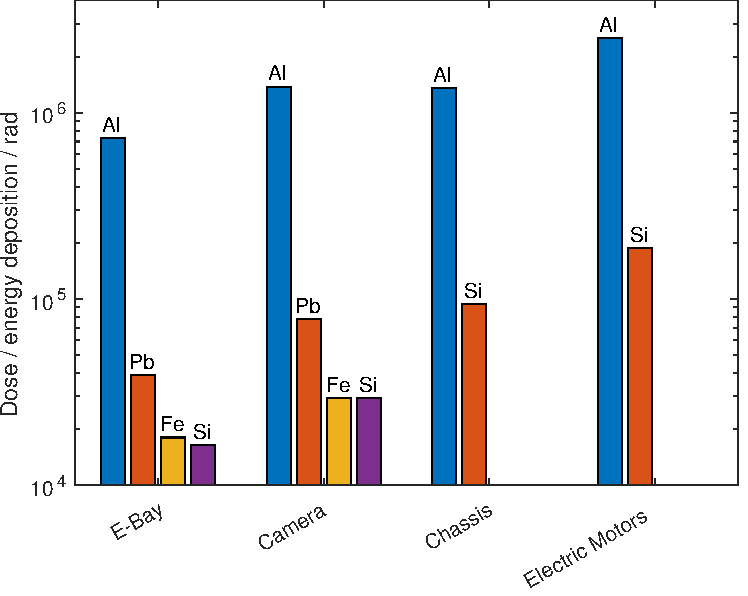
\includegraphics[width=\textwidth]{Media/J_Electron_Compartments}
         \caption{TID for Electrons as Source Particles}
         \label{fig:TIDElectronShielding}
     \end{subfigure}
     \hfill
     \begin{subfigure}[b]{0.49\textwidth}
         \centering
         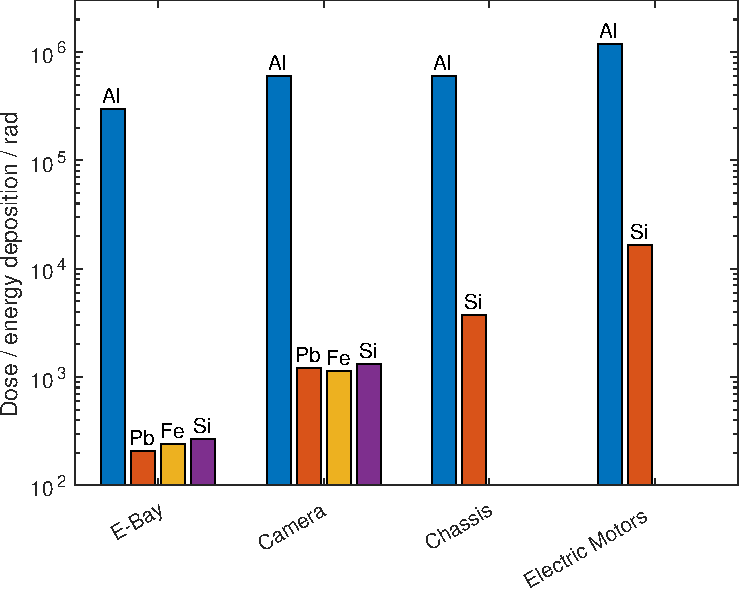
\includegraphics[width=\textwidth]{Media/J_Proton_Compartments}
         \caption{TID for Proton as Source Particles}
         \label{fig:TIDProtonShielding}
     \end{subfigure}
     \caption{TID for different compartments as seen in \autoref{fig:RadiationOverview}. The E-Bay is shielded by 4 mm aluminium, 0.415 mm lead, and 0.033 mm iron; the camera compartment by 2 mm aluminium, 0.415 mm lead, and 0.033 mm iron; the chassis by 2 mm aluminium; the electric motors by 1 mm aluminium.}
     \label{fig:CompartmentTID}
\end{figure}

\newpage

\subsection{Improvements}

\label{app:AppendixRadiationImprovements}

All simulations of the improvements introduced in \autoref{subsec:RadiationImprovements} are performed in the same way as in \autoref{subsec:AppendixRadiationExposures}. \\ \\
In \autoref{fig:Radiation_Improvements_Individual}, the TID over 30 days within the E-Bay is shown. If all components with a radiation resistance under 43.27 krad are shielded individually, the additional shielding structure around the E-Bay can be removed and the aluminium structure would be sufficient.

\begin{figure}[htp]
	\centering
	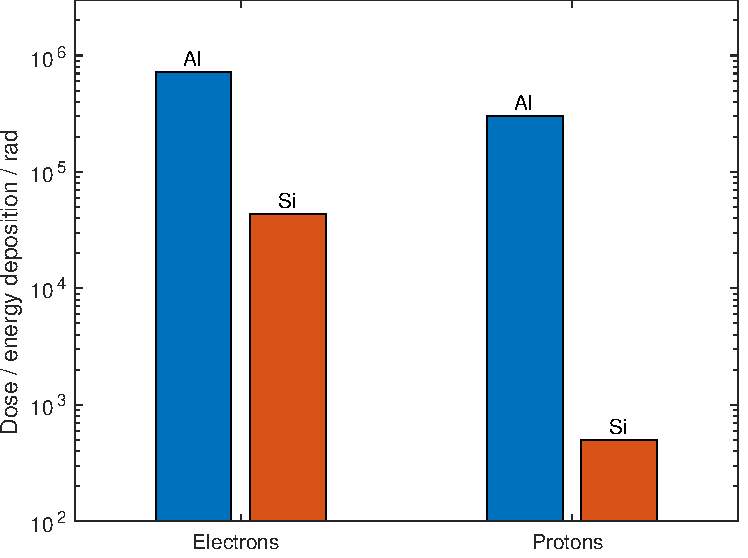
\includegraphics[width=0.7\textwidth]{Media/J_Improvements_Individual}
	\caption{TID with 4 mm Al shielding over a mission duration of 30 days}
	\label{fig:Radiation_Improvements_Individual}
\end{figure}

The resulting mass savings can be calculated with \autoref{eq:RadiationImprovementsIndividual} with \(m^*\) as the specific weight of the radiation protection and \(N\) as the amount of components within the E-Bay with a radiation resistance under 43.27 krad as of \autoref{tab:RadiationList}.

\begin{equation}
	\Delta m = SA_\text{E-Bay} \cdot m^*_\text{Shielding} - \sum\nolimits_{n=0}^N SA_\text{Component, n} \cdot m^*_\text{Shielding}
	\label{eq:RadiationImprovementsIndividual}
\end{equation}

With inserted values this results in a mass saving of \(\Delta m\) = 736.2 g.

\begin{figure}[htp]
	\centering
	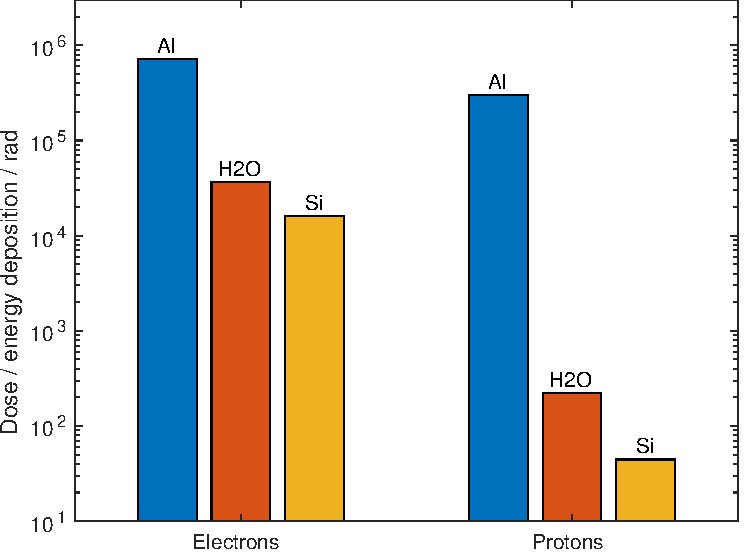
\includegraphics[width=0.7\textwidth]{Media/J_Improvements_Ice}
	\caption{TID with 4 mm Al shielding and 1 cm of Water over a mission duration of 30 days}
	\label{fig:Radiation_Improvements_Ice}
\end{figure}

\clearpage

\setcounter{figure}{0}
\setcounter{table}{0}

%-----------------------------------------------------------
\section{Digital Appendix}		\label{app:DigitalAppendix}
%-----------------------------------------------------------

\begin{table}[htb]
	\centering
	\begin{tabular}{llcc}
		\hline
		Name  & Path & Type & Size  \\ \hline
		TCS Analysis final & \300 Thermal\ & Exle Sheet with Macros, *.xlsm & 326 kB  \\   \hline
	\end{tabular}
\end{table}

\cleardoublepage